\chapter{Эксперимент NA64}

Рассмотрим применение описанных принципов проектирования
научного~\acrshort{sw} на примере эксперимента NA64.
%Название коллаборации по внутренней номенклатуре экспериментов Европейской организации по
%ядерным исследованиям (North Area, №64).

Программа эксперимента посвящёна поиску гипотетических частиц тёмной материи в
постановке <<active beam dump>>, где
наблюдается развитие электромагнитного ливня от лептона в веществе активной мишени
($e^{-} + Z_{\text{Pb}}$, $\mu^{-} + Z_{\text{Pb}}$, $e^{+} + Z_{\text{Pb}}$).
NA64 нацелен на проверку различных моделей \acrshort{dm}, включая скалярные
частицы, псевдоскаляры, майорановскую тёмную материю: тёмный фотон,
лёгкие аксион-подобные частицы, инфлатон и $Z'$-бозон.

%В этой главе дано краткое
%описание экспериментальной установки, приведены примеры конкретных
%реализаций общих принципов изложенных ранее.

%Вне зависимости от конкретного гипотетического механизма,
%эксперимент существенным образом опирается на информацию об электромагнитном 
%ливне, индуцированным налетающим на мишень лептоном. 
%Такую информацию регистрирует гетерогенный электромагнитный калориметр с высокой
%гранулярностью (\texttt{ECAL}), играя таким образом особую роль
%в рамках экспериментальных методов регистрации гипотетических каналов реакции.
%По этой причине, особое внимание в главе уделяется задачам калибровки и
%реконструкции сигналов электромагнитного калориметра.

\section{Сигнальные процессы}

\subsection{Тёмный фотон}

Одним из популярных гипотетических механизмов описания связи \acrshort{dm}
с физикой СМ является расширение групп симметрии 
лагранжиана СМ путем добавления абелевой калибровочной группы $U_D(1)$, 
действующей в секторе темной материи~\cite{holdom} и кинетически смешанной 
с абелевой электромагнитной группой $U_{\textrm em}(1)$:
\begin{equation}
\label{LCM_A}
    \mathcal{L}_{SM+A'} = \mathcal{L}_{SM} + \epsilon \, F^{\mu\nu} F'_{\mu \nu}
        - \frac{1}{4} F'^{\mu\nu} F'_{\mu\nu} + \frac{m_{A'}^2}{2} m_{A'}^2 A'^{\mu}A'_{\mu},
\end{equation}
где
% совет: "должна быть полная расшифровка всех величин"
$\mathcal{L}_{SM}$ --- лагранжиан \acrshort{sm}, 
$A'_{\mu}$ и $m_{A'}$ --- полевой оператор и масса тёмного фотона, 
который является массивным векторным бозоном, 
$F_{\mu \nu}$ и $F'_{\mu \nu}$ --- тензоры напряженности 
электромагнитного поля (фотона) и поля тёмного фотона, соответственно,
$\epsilon_Y$ --- константа взаимодействия  
электромагнитного поля и поля темного бозона. 

% NOTE  ГОСТ Р2 . 105 - 2019:
%       "Пояснения символов и числовых коэффициентов, входящих в формулу, если
%       они не пояснены ранее в тексте, должны быть приведены непосредственно
%       под формулой. Пояснения каждого символа следует давать с новой строки
%       в той последовательности, в которой символы приведе
%       ны в формуле. Первая строка пояснения должна начинаться со слова
%       «где» без двоеточия после него."
% при этом:
% NOTE  В ГОСТах, регламентирующих оформление научной и технической документации
%       (например, ГОСТ 7.32-2001 и ГОСТ 2.105-95, знаки пунктуации в конце
%       отдельно стоящих формул _указываются_)

Далее в лагранжиане~(\ref{LCM_A}) вводится взаимодействие тёмного 
фотона с фермионами \acrshort{sm} $\psi$:
\begin{equation}
\label{L_Apsi}
    \mathcal{L}_{A\bar\psi\psi} = \epsilon \, A'_\mu  
    \bar\psi \gamma^\mu Q_\psi \psi 
\end{equation}
где $Q_\psi$ --- электрический заряд СМ фермиона (заряженный лептон или кварк), 
производя сдвиг электромагнитного поля 
$A_\mu(x) \to A_\mu(x) + \epsilon \, A'_\mu(x)$, который также устраняет 
смешивание наблюдаемого и темного фотона, т.е. член 
$\epsilon \, F^{\mu\nu} F'_{\mu \nu}$.

Экспериментальное наблюдение взаимодействия описанного
лагранжианом~\eqref{LCM_A} может быть произведено, например,
в реакции фотообразования при рассеянии
электрона на тяжёлом ядре, изображённой на рисунке \ref{fig:aprime-production}.
Интегрирование матрицы рассеяния позволяет получить приблизительные
количественные оценки для постановки таких экспериментов на
ускорителях обеспечивающих энергию лептонов порядка
нескольких сотен ГэВ.

\subsection{Лёгкие аксион-подобные частицы}

Наряду с тёмным фотоном в литературе существует другой хорошо мотивированный 
тип частиц новой физики --
аксион-подобные частицы $a$~(\emph{axion-like particles} --ALPs)~\cite{Dobrich2016}), 
предложеных Пессей-Куинн~\cite{Peccei:1977hh}, Вайнбергом~\cite{Weinberg:1977ma} 
и Вильчеком~\cite{Wilczek:1977pj} 50 лет назад. 

%\begin{wrapfigure}{r}{0.35\textwidth}
\begin{figure}
    \centering
    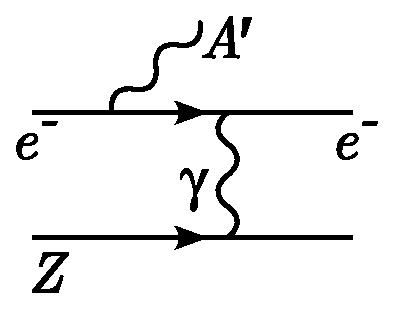
\includegraphics[width=.55\linewidth]{images/illustrative/aprime-photoprod.eps}
    \caption{Фоторождение $A'$ на ядре $Z$}
    \label{fig:aprime-production}
\end{figure}
%\end{wrapfigure}

Постулируя, что $a$ является псевдоскалярной частицей, можно построить 
феноменологический лагранжиан, описывающий его свободное движение и взаимодействие 
с электромагнитным полем 
\begin{equation}
    \mathcal{L}_{F+a} = - \frac{1}{4} g_{a \gamma \gamma} a F_{\mu \nu} \tilde F_{\mu \nu}
        + \frac{1}{2} (\partial_{\mu} a)^2 - \frac{1}{2} m^2_a a^2,
\end{equation}
где $\tilde{F}_{\mu \nu} = \frac{1}{2} \epsilon_{\mu \nu \lambda \rho} F^{\lambda \rho}$ --- дуальный тензор электромагнитного поля,
$g_{a \gamma \gamma}$ -- константа связи, и $m_a$ -- масса ALP частицы.

Эксперимент по поиску $a$ подразумевает постановку схожую с экспериментом
по поиску $A'$. Диаграмма реакций приведена на рисунке~\ref{fig:axion-photo}.

\begin{figure}[ht]
    \centering
    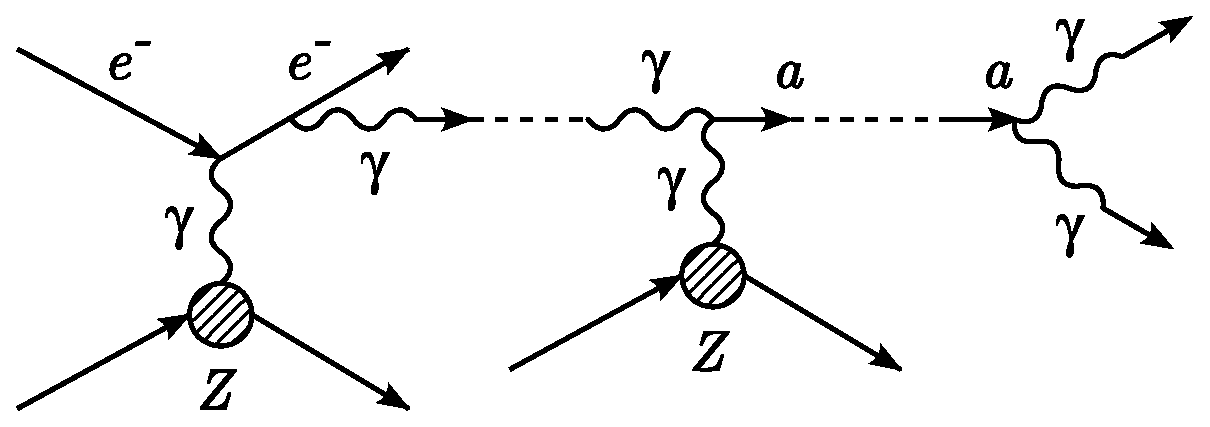
\includegraphics[width=0.75\linewidth]{images/illustrative/ALPs-photoprod-ours.eps}
    \caption{Фоторождение и распад аксион-подобной частицы (ALP).}
    \label{fig:axion-photo}
\end{figure}
\section{Постановка эксперимента}

Эксперимент NA64 (а также его <<мюонная версия>>, получившая название
NA64mu) использует постановку <<\emph{active beam dump}>> в рамках
которой массивная мишень сама по себе является детектором, а в конкретном
случае NA64 -- гетерогенным (свинец-полиметилметакрилат) электромагнитным
калориметром высокой гранулярности ECAL.

\subsection{Описание установки}

Начатый в 2015-ом году, эксперимент NA64 изначально
был направлен на поиск лёгкого бозона $A'$ получившего в литературе название
<<\emph{тёмный фотон}>> из-за того что гипотетическим механизмом его
образования является редкая конверсия посредством механизма электромагнитного
смешивания, которую можно описать через соответствующую добавку к
электромагнитному слагаемому лагранжиана \acrshort{sm}.

Экспериментальная установка для поиска $A'$ по недостающей энергии
в упрощённом виде изображена на рисунке \ref{fig:setup-schematic-invis}.
Установка состоит из двух калориметров -- электромагнитного
гетерогенного (сэмплирующего) калориметра ECAL, играющего роль активной мишени,
и адронного гетерогенного
калориметра HCAL. Установка снабжена системой мечения частиц, состоящей из
двухплечевого спектрометра на основе газовых микроструктурных трековых
детекторов T1-T4, измеряющих отклонение электронов в поле
магнита~($1.5\text{Тл}$). Триггерная система в простейшем случае
состоит из телескопа быстрых сцинтилляционных счётчиков S1, S2, S3.
Вето-детектор V1 и мюонный счётчик MU1 включаются в триггер в
режиме антисовпадений для исключения гало пучка и подавления мюонного
фона.

\begin{figure}
    \centering
    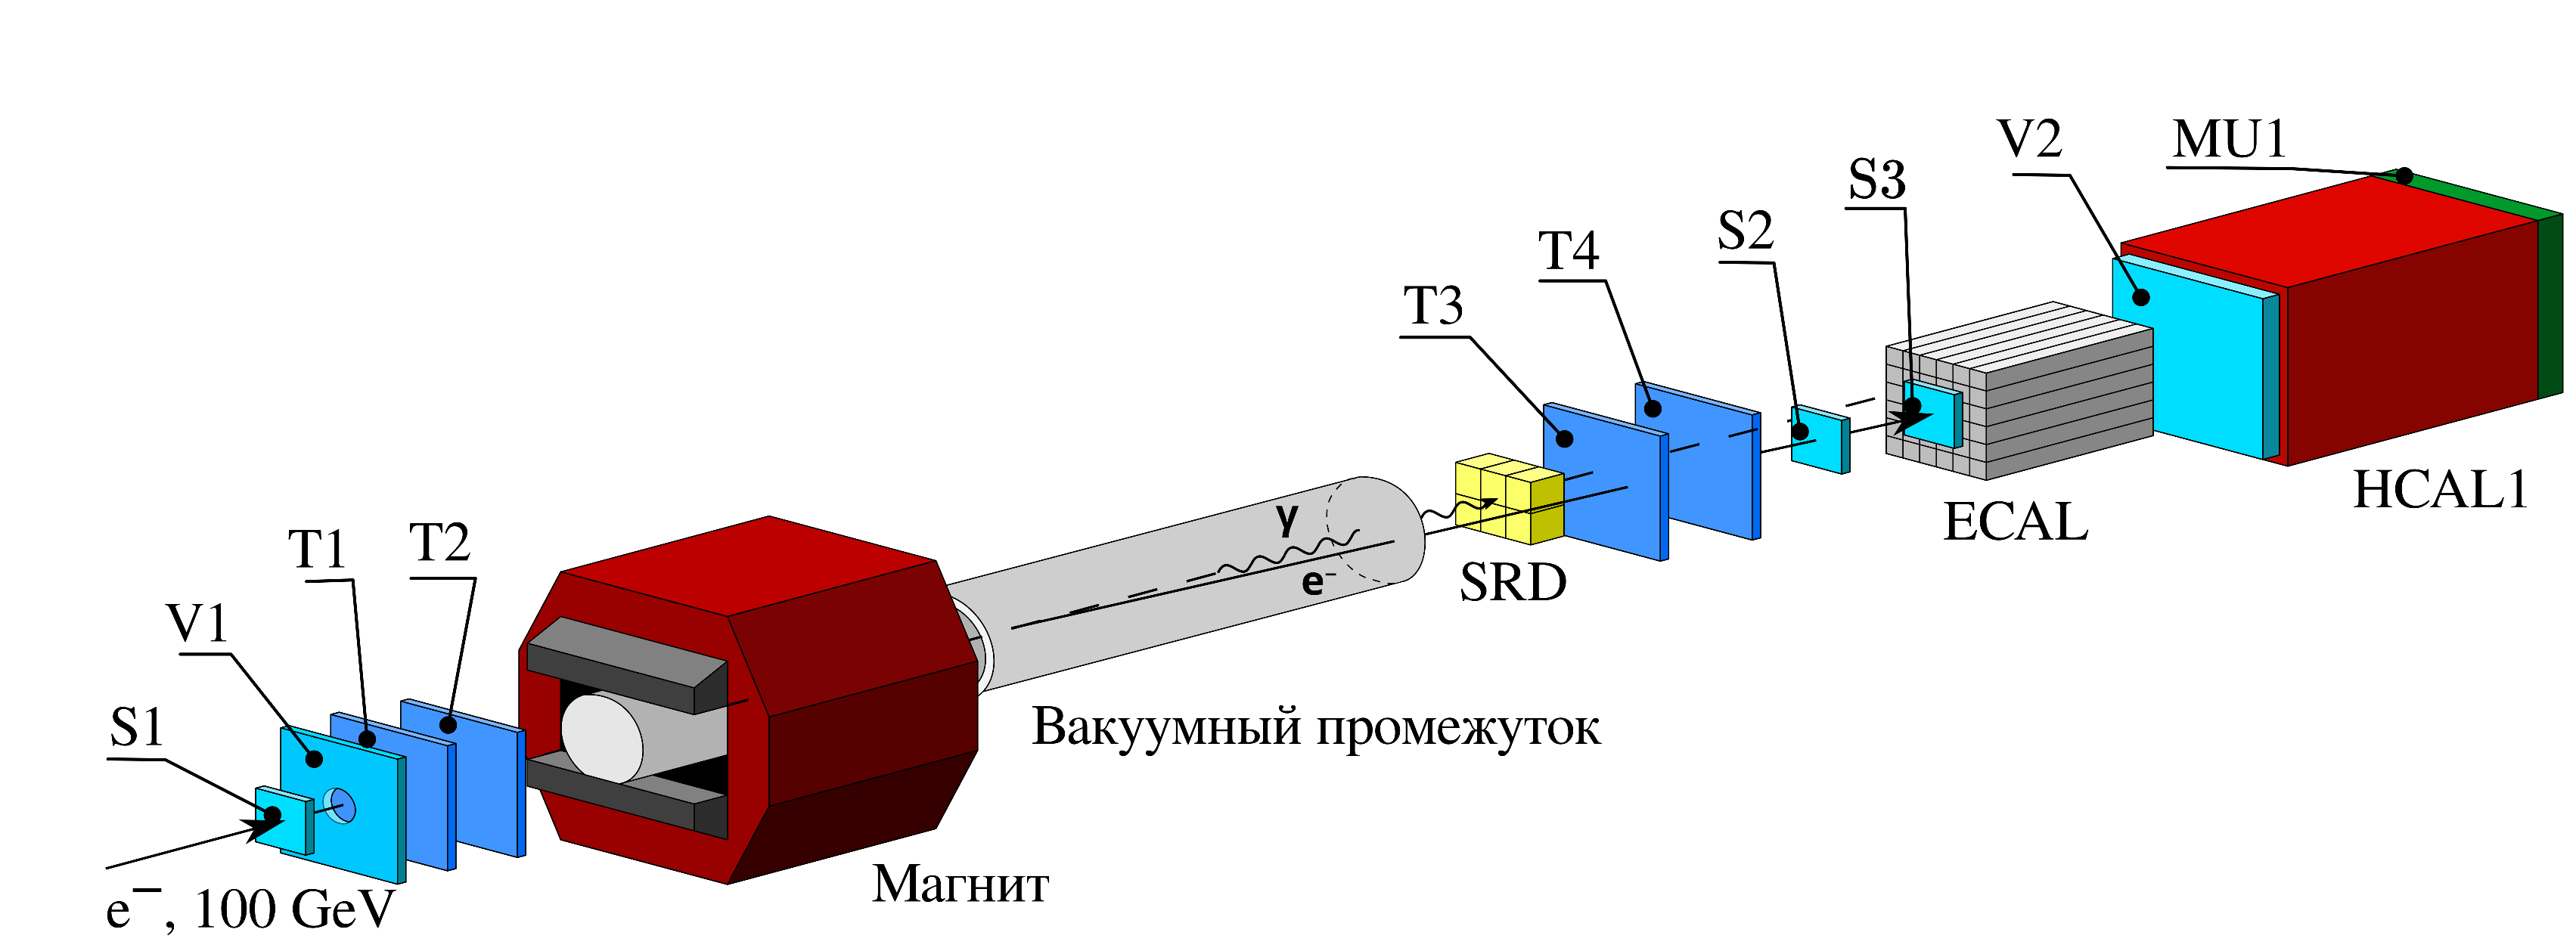
\includegraphics[width=1\linewidth]{images/illustrative/setup-schematic.eps}
    \caption{Размещение детекторов установки NA64 в постановке для обнаружения невидимых частиц}
    \label{fig:setup-schematic-invis}
\end{figure}

Поиск по недостающей энергии заключается в регистрации таких событий,
когда в обоих калориметрах отсутствует существенная часть энергии
инициирующей частицы (несколько десятков ГэВ), что соответствует
образованию высокоэнергетической частицы, способной покинуть
установку без взаимодействия.

Нужно заметить, что ряд процессов \acrshort{sm} в теории способны
реализовать такую сигнатуру: т.н. проникающие (<<пробивные>>,
англ. \emph{punchthrough}) фотоны, нейтральные частицы, мюоны,
альбедо-рассеяние частиц в первых нескольких актах взаимодействия в
мишени и т.д. NA64 оценивает вероятность таких событий менее $10^{-12}$,
что определяет нижний порог чувствительности установки к реакциям такого
типа.

Изображённая на рисунке~\ref{fig:setup-schematic-invis} постановка
может быть существенно модифицирована. Например, с целью подавления фоновых
каналов вместо сцинтилляционного детектора V1 для исключения
адронной компоненты фона в эксперимент в 2018г. были введены сэмплирующие
медные вето-калориметры, трекер дополнен несколькими дополнительными
микропаттерными детекторами и трубчатыми дрейфовыми
детекторами~(\emph{straw}-станциями). Для оценки мюонных фонов
straw-станции низкого разрешения расположены позади адронного калориметра.
В реальности, калориметр HCAL имеет продольную сегментацию, и состоит из
четырёх независимых модулей с поперечной сегментацией $3\times 3$ для
приближённой оценки профиля адронного ливня.

В качестве детектора синхротронного излучения (SRD) в разное время применялись
сегментированные калориметры BGO (из германата висмута), LYSO (ортосиликат
лютеция легированный церием), а так же вольфрам-пластиковые ячейки близкие
по составу к элементам электромагнитного калориметра ECAL.

% TODO: ECAL radiation length
% In order to measure direction of e/m shower and provide good \pi_0 rejection
% (why?) a preshower detector would be required at CMS --- shashlik proposal
% 1993
% TODO: HCAL radiation length

\subsection{Получение пучков и номенклатура данных}

Источником пучка выосокэнергетических ($100~\text{ГэВ}$) электронов в
эксперименте NA64 является ускоритель SPS (\emph{Super Proton
Synchrotron} – протонный суперсинхротрон). Вокруг ускорителя расположены
несколько экспериментальных зон. Эксперимент NA64 проводится в
Северной зоне (\emph{North Area}), включающей в себя два наземных
и один подземный залы, в которых размещены несколько станций вывода
пучка. На этих станциях пучок может выводиться напрямую в зону
эксперимента, либо направляться на мишень-конвертер для генерации пучка
вторичных частиц. Установка NA64 развёрнута на площадке H4,
предоставляющей электронный и адронные пучки. Для
реализации программы NA64mu, оборудование эксперимента перемещается на
площадку M2.

\subsubsection{Конверсия протонов пучка SPS}

В постановке на электронах NA64, пучок протонов с энергией $450~\text{ГэВ}$
интенсивностью $1{,}5 \times 10^{12}$ протонов/на период сбрасывается
на бериллиевую мишень, откуда пучок вторичных частиц передается в
тракт H4, состоящий из набора коллиматоров, отклоняющих и фокусирующих
магнитов, обеспечивающих малый разброс по энергиям и высокую чистоту пучка.

Первичная мишень представляет собой набор из пяти бериллиевых пластин
различной толщины. Толщины пластин составляют 40, 100, 180, 300 и 500~мм.
Пластины установлены в подвижном корпусе окруженном защитой. Соотношение
доли электронов к адронам в конверсионном ливне растет линейно с
увеличением длины мишени. Вторичные адроны образуются в реакциях вида
$p + Z \rightarrow H$ и их доля растёт в линейной пропорции к толщине
мишени $L$, в то время как вторичные электроны в основном являются результатом
распада адронов в реакциях
вида~$p + X \rightarrow \pi^0 \rightarrow \gamma \gamma$, где
аннигиляционные кванты $\gamma$ затем образуют в материале мишени
$e^{+}e^{-}$-пары. Часть из них, пропорциональная $e^{-L}$ поглощается
в веществе мишени. Таким образом, отношение полного выхода электронов и
адронов в конвертере пропорционально $L$ ($L^2 e^{-L}/L e^{-L} = L$),
что позволяет осуществлять эффективную конверсию и сепарацию вторичных
электронов в тракте H4.

Ускорительный комплекс SPS производит вывод пучка периодически --
с периодом в несколько десятков секунд (называемых \emph{суперциклом}),
в течение которых чередуются этапы накопления и сброса пучка.
Сброс пучка длится несколько секунд, остальное время происходит
накопление протонных сгустков в ускорительной ситсеме.

\subsubsection{Номенклатура данных}

К механизму накопления и сброса пучка ускорителя SPS привязана
идентификация событий в данных NA64.

Наиболее общей временной отметкой является отдельный
\emph{экспериментальный сеанс} в течение которого набор
детекторов установки и их взаимное геометрическое расположение
остаются в большой степени неизменными. В течение сеанса
процедуры настройки, калибровки и геометрической юстировки
детекторов производятся заново, обычно в несколько этапов.

С точки зрения накопленных данных, сеансы делятся на набор
пронумерованных подряд \emph{ранов} (англ.~\emph{run}) --
периодов набора статистики с типичной
продолжительностью в один или два часа, в течение которых
экспериментальный зал закрыт и условия набора данных предполагаются
постоянными. Номер рана остаётся уникальным в течение всего
жизненного цикла эксперимента.

Начало и конец рана выдерживаются привязанными к числу актов
сбросов пучка ускорителем. Временной интервал в течение которого
производится квазинепрерывный (банчированный) вывод пучка
называется~\emph{спилл}~(англ. \emph{spill}). Спиллы нумеруются
в ране подряд, и таким образом номер спилла в ране остаётся
уникальным.

Наконец, в пределах одного спилла, нумеруются подряд отдельные
события зарегистрированные триггером.

Таким образом, три числа обозначающие
\begin{itemize}
    \item Номер рана,
    \item Номер спилла,
    \item Номер события в спилле
\end{itemize}
составляют уникальный идентификатор события, который следует
использовать в программной базе эксперимента.

Ожидается, что число ранов NA64 не превысит $10^7$, число
спиллов в ране не превышает $10^3$, а число событий в одном
принципиально ограничено $10^9$. Таким образом, тип данных
для обозначения события потребует мощности в $10^19$ уникальных
значений, что позволяет кодировать идентификатор события
64-разрядным целым числом~($2^{64} \simeq1.85\times10^{19}$),
с сохранением семантики <<ран, спилл, номер события>>.

\section{Детекторы}

\subsection{Электромагнитный калориметр}

Оригинальная идея считывать свет из слоистого калориметра посредством
спектросмещающих волокон (WLS) предложена в 1985 году Фесслером \cite{Fessler-Shashlik-1985}.
Идея была впервые реализована в виде гетерогенного ячеистого калориметра в
1991-1992 годах в ИЯИ РАН для эксперимента E-865~(BNL, США) \cite{BADIER199474}.
% ^^^ проверить, впервые ли -- доклад Гущина (см. слайд №5) выглядит
% пристрастным: http://www.inr.troitsk.ru/rus/kud-sem/gushchin26-03-12.pdf
% Встречал упоминание о гетерогенном калориметре CDF (Fermilab), 1988, где
% при толщине 18 X_0 Pb/scint разрешение составляло 13.5%/\sqrt{E}
% KLOE использовали 15 X_0 с файберами в 1995 5.7%/\sqrt{E} + .6%
В последующие годы калориметры такого типа получили широкое распространение за
счёт ряда технологических преимуществ~\cite{grupenDetectors2008}.
К числу таких преимуществ относятся:
\begin{itemize}
    \item Возможность создания калориметра под необходимый мольеровский радиус,
    позволяющий производить пространственное разделение ливней от различных частиц, \item высокая радиационная стойкость, устойчивость отклика при работе в магнитном поле,
    \item стабильное энергетическое разрешение и высокая скорость отклика во
    многих случаях позволявшая включать такой калориметр в триггерную систему.
\end{itemize}

Идея нашла применение во многих экспериментах.
%:PHENIX (BNL), LHCb, DELPHI, CMS, COMPASS (CERN), HERA-B (DESY) и т.д.
С 1993 по 2003 годы в CERN действовала коллаборация посвящённая
развитию детекторов такого типа для задач эксперимента
CMS --- RD36~\cite{rd36-shashlik-1996}.
%Работы RD36 послужат методической основой для предлагаемой в
%настоящей диссертации процедуры калибровки ECAL \cite{rd36-shashlik-1996}.
% R&D proposal of 1993 https://cds.cern.ch/record/293003/files/SC00000220.pdf :
%   a = 8.4 +/- 1, c = .37 +/- .3, b = .8 +/- .2
%   \sigma_{mrad} = 70 / \sqrt{E}.
% 8.1  0.5  0.33

Калориметр NA64 представляет собой прямоугольный сегментированный блок, ячейки
которого конструктивно схожи с использованными в RD36 и COMPASS,
%ECAL NA64 имеет сегментацию, размеры ячеек, толщины слоёв и
%размещение оптического волокна.
Ячейки состоят из пластин свинца и
полиметилметакрилата (\acrshort{pmma})
набранных на стальные стержни для обеспечения механической
прочности с проходящим вдоль ячейки оптическим волокном имеющим оптический
контакт с пластинами сцинтиллятора.
Поперечная сегментация калориметра -- $6 \times 6$ или $5 \times 6$ квадратных
ячеек со стороной $38.2~\text{мм}$.
В продольном направлении калориметр разделён на предливневую и основную
части. На рисунке~\ref{fig:ecal-assembly-photo-opened} приведена фотография
торцевой части калориметра $6 \times 6$ в процессе установки светопроводящих
волокон, которые можно видеть в нижней части рисунка. торцы волокон от каждой
ячейки зачищаются и сводятся в пучок на катоде одного фотоприёмника.
\begin{figure}[h]
    \centering
    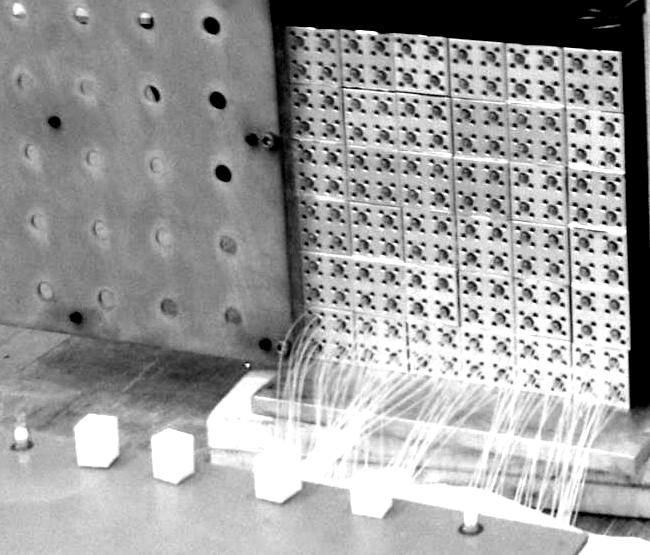
\includegraphics[width=0.5\linewidth]{images/illustrative/ecal-assembly-photo-opened.png}
    \caption{Фотография торцевой части ECAL NA64 со снятым кожухом}
    \label{fig:ecal-assembly-photo-opened}
\end{figure}
Свинцовые пластины имеют толщину~$1.5~\text{мм}$,
пластины из \acrshort{pmma} имеют толщину $1.55~\text{мм}$.
Для предохранения поверхности сцинтиллятора от механического
воздействия между ними вводится бумажная проставка толщиной $140~\text{мкм}$.
Предливневая часть состоит из 16-и слоёв, основная часть из 150-и.
Все пластины имеют перфорацию для пропускания светопроводящего волокна
(16 отверстий на ячейку) и армирующих стальных стержней (четыре отверстия).

Таким образом, калориметр имеет толщину соответствующую примерно 42
радиационным длинам ($\simeq42{,}4 X_0$) и мольеровский
радиус~$R_M\simeq1{,}8~\text{см}$, откуда следует, что при попадании
электрона в калориметр, его энергия
за счёт одного только тормозного излучения уменьшится в $e^{42}$ раз.
Практически, высокоэнергетический электрон инициирует
в веществе калориметра развитие электромагнитного ливня (каскада) за
счёт процессов образования пар, комптоновского рассеяния и
фотоэлектрического эффекта. 90\% энерговыделения сосредоточено
внутри цилиндрического объёма диаметром $36~\text{мм}$ -- в одной
ячейке в случае центрального падения.

Для задач калибровки калориметра важно, что \acrshort{mip} для
мюонов с энергией свыше нескольких десятков ГэВ
составляет $\simeq353~\text{МэВ}$ ($2{,}26~\text{МэВ}$ на слой).

%На рисунке приведена визуализация моделирования образования
%электромагнитного ливня в ECAL и профиль ливня \cite{grupenDetectors2008}
%Сигнал от предливневой части вводится в триггерную систему и служит в основном
%для отделения адронных событий.

Энергетическое разрешение калориметров определяется следующей
формулой, учитывающую вклад отдельных свойств детектора и считывающей системы:
% (символом "$\oplus$" обозначена прямая сумма)
\begin{equation}
    \frac{\sigma}{E} = \frac{a}{\sqrt{E}} \oplus b \oplus \frac{c}{E}.
    \label{eq:ecalResolution}
\end{equation}
В формулу включены феноменологические параметры $a, b, c$, отвечающие за
влияние эффектов различной природы \cite{CalorimetryPPhFabiola}:
\begin{itemize}
    \item $a$ -- стохастический член, отвечающий за фотостатистику,
    в который включены внутренние флуктуации в ливне, флуктуации
    в отдельных слоях и квантовые флуктуации сигнала,
    \item $b$ -- постоянный член отвечающий за флуктуации
    электроники (динодная система, зарядово-цифровые или
    амплитудно-цифровые преобразователи и т.д.),
    \item $c$ -- слагаемое отвечающее за ошибки калибровки,
    неоднородности сцинтиллятора и другие независящие от энергии
    факторы.
\end{itemize}

Для гетерогенных калориметров типичное относительное
энергетическое разрешение лежит в
диапазоне~$5-20\%/\sqrt{E}$~\cite{CalorimetryPPhFabiola}.
При этом считается, что основной вклад в
ухудшение разрешения вносят флуктуации в отдельном активном слое (число
заряженных частиц $n_{ch} \propto E/t$, где $t$ -- толщина слоя
поглотителя)~\cite{grupenDetectors2008, wigmansCalorimetry},
при этом стохастический член $a$ из $\eqref{eq:ecalResolution}$
изменяется как $\sigma_{samp}/E \propto \sqrt{t/E}$.
С целью её уменьшения стремятся увеличивать число слоёв,
уменьшая толщину отдельного слоя поглотителя.

В частности, чтобы получить представление о значениях энергетического
(а также координатного и углового) разрешения достижимых
практически в калориметре конструктивно-схожего типа, можно
обратиться к работам RD36. В техническом проекте~\cite{rd36-shashlik-1996}
приводятся оценки для калориметра свинец-полиметилметакрилат с
толщинами слоёв~$2~\text{мм}$ и $4~\text{мм}$ соответственно, и
стороной ячейки~$47~\text{мм}$. В этой работе отмечается сильная
зависимость энергетического разрешения ячейки калориметра от
координаты попадания первичной частицы
(рисунок~\ref{fig:shashlyk-correction-quote}, слева). С целью
компенсации эффекта,
вводится феноменологическая аппроксимация оценки энерговыделения
как функция координаты попадания первичной частицы, результаты которой
представлены на рисунке~\ref{fig:shashlyk-correction-quote}.

С учётом координатной коррекции, авторы указывают энергетическое
разрешение для случая, когда выход считывается
высокостабильным~\acrshort{pmt}
\begin{equation}
    \frac{\sigma}{E}(\%) = \frac{9.0 \pm 0.1}{\sqrt{E}} \oplus (1.0\pm0.3),
\end{equation}
т.е. для электрона~$100~\text{ГэВ}$ принципиальный предел энергетического
разрешения составляет~$\sigma =1.9~\text{ГэВ}$.

\begin{figure}
    \centering
    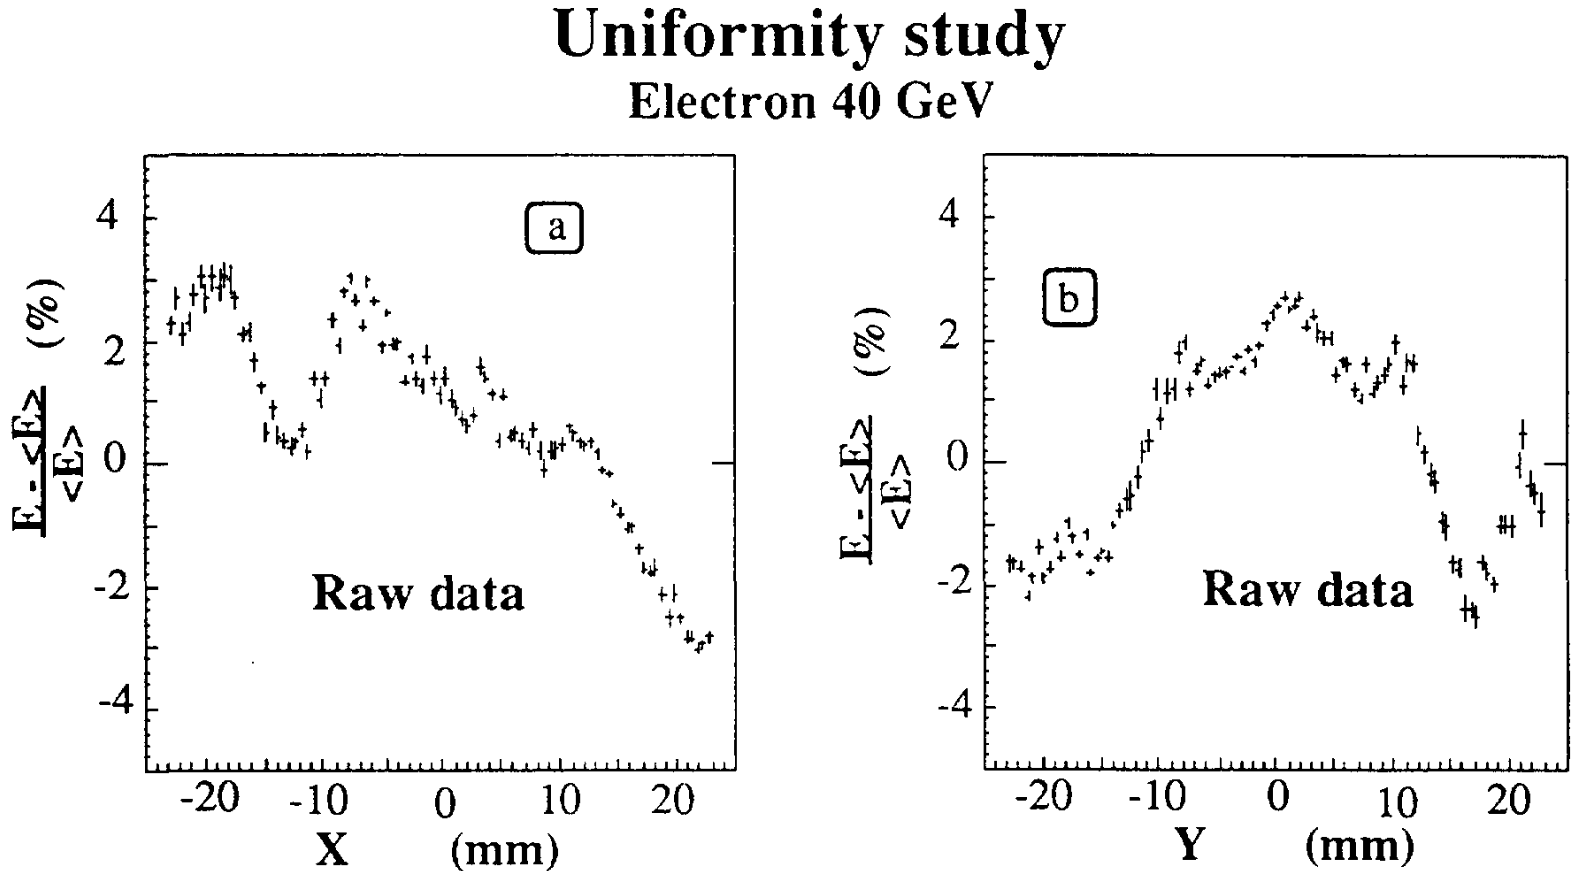
\includegraphics[width=0.48\linewidth]{images//illustrative/shashlyk-resolution-raw.png}
    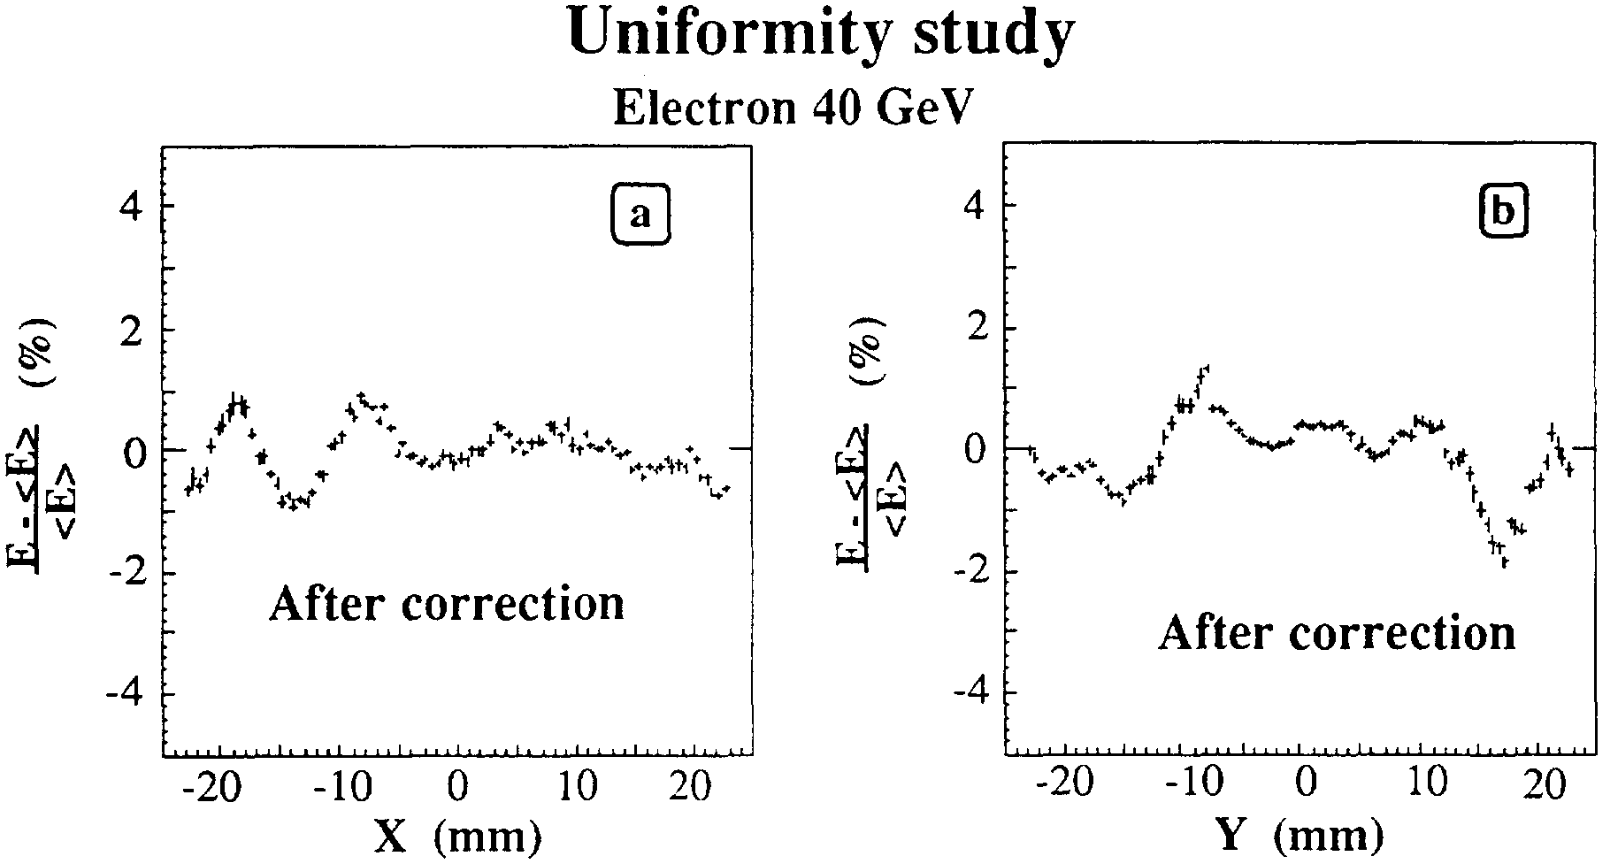
\includegraphics[width=0.48\linewidth]{images//illustrative/shashlyk-resolution-corrected.png}
    \caption{Зависимость оценки энерговыделения калориметра от координаты до и после коррекции согласно работе~\cite{rd36-shashlik-1996}}
    \label{fig:shashlyk-correction-quote}
\end{figure}

Результаты измерения энергетического разрешения
конструктивно-аналогичного калориметра опубликованы
в работе~\cite{chirkovzorin-compass-ecal}. За исключением
фотоприёмника и числа слоёв,
калориметр~COMPASS использует аналогичную NA64 конструкцию
ячеек, включая поперечные размеры, толщины слоёв, марку оптического
волокна и т.д. Полученная зависимость изображена на
рисунке~\ref{fig:chirkovzorin-compass-ecal}.
\begin{figure}
    \centering
    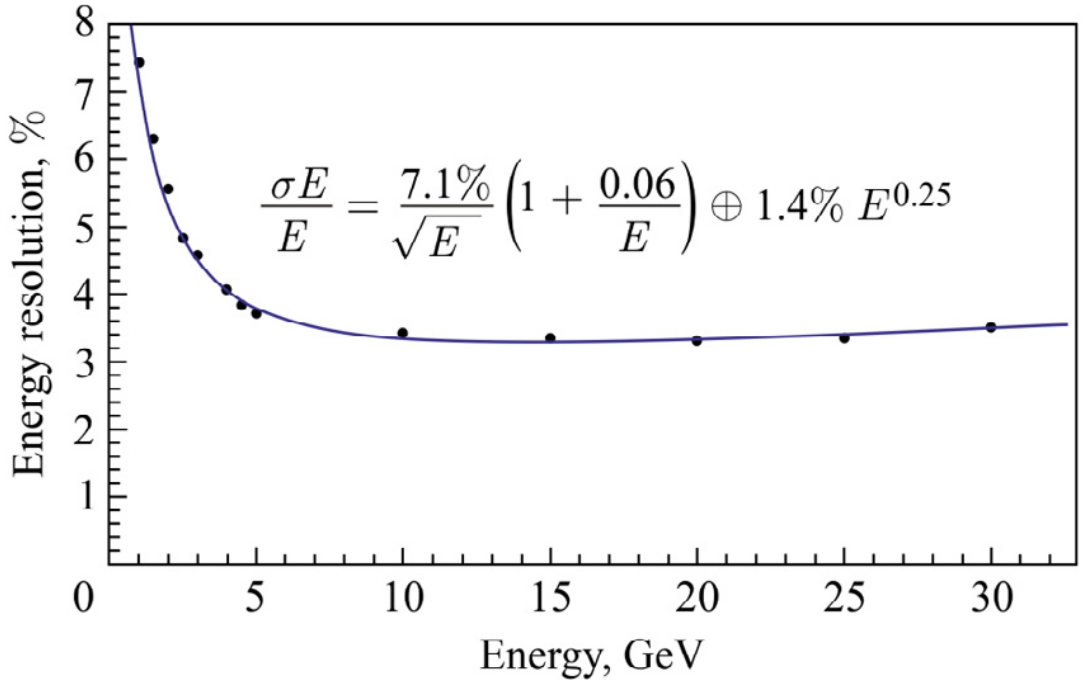
\includegraphics[width=0.5\linewidth]{images//illustrative/compassII-ecal.png}
    \caption{Относительное разрешение ECAL COMPASS фазы II, согласно~\cite{chirkovzorin-compass-ecal}}
    \label{fig:chirkovzorin-compass-ecal}
\end{figure}

Экстраполяция оценки относительного разрешения из этой работы до номинальной
энергии пучка NA64 ($100~\text{ГэВ}$) даёт значение $\simeq 5{,}14~\text{ГэВ}$.
Следует учесть, что практически разрешение должно быть несколько лучше,
поскольку линейный член в работе~\cite{chirkovzorin-compass-ecal}
отвечает за флуктуацию продольных утечек (и обуславливает ухудшение
относительного разрешения на рисунке~\ref{fig:chirkovzorin-compass-ecal}.

%---

%Для апостериорного вычисления коэффициентов
%выражения~\eqref{eq:ecalResolution}, прямая сумма $\oplus$ раскрывается
%следующим образом:
%\begin{equation}
%    \frac{\sigma (E)}{\langle E \rangle} = \sqrt{ \frac{c^2}{\langle E \rangle} + \frac{b^2}{\langle E \rangle^2} + \left( \frac{\sigma(p)}{p} \right)^2 },
%\end{equation}
%где $\sigma(p)/p$ --- импульсное разрешение установки.
% ^^^ проверить, взял https://arxiv.org/abs/hep-ex/0001020 , стр 11, ф-ла (42)

%Текущий раздел будет посвящён отысканию коэффициентов в
%формуле \eqref{eq:ecalResolution} и созданию параметрической модели
%электромагнитного ливня для дальнейших приложений.

\subsection{Адронный калориметр}

В качестве адронного калориметра в NA64 установлен
нескомпенсированный калориметр железо-\acrshort{pmma}.
Калориметр имеет поперечную сегментацию $3\times3$
и состоит из четырёх независимых модулей. В рассматриваемых
в данной работе постановках эти модуле, как правило, ориентируются
вдоль по оси пучка и устанавливаются подряд, совместно с ECAL
образуя герметичный детектор.

Конструктивно, каждый модуль калориметра выполнен в виде
сварной металлической конструкции, в которую помещаются
вкладыши со сборками сцинтилляционных пластин из \acrshort{pmma}
обёрнутых в металлизированный майлар, с выведенными наружу
сцинтилляционными волокнами, как показано на рисунке~\ref{fig:hcal-module}.

Толщина одной $192\times194~\text{мм}$ сцинтилляционной
пластины -- $4~\text{мм}$, поглотителя -- $25~\text{мм}$.
Во вкладыше пластины расположены с небольшим зазором для обеспечения
выхода волокна, так что общая длина одного модуля калориметра
состоящего из 48-и слоёв составляет $1500~\text{мм}$, обеспечивая,
таким образом длину ядерного взаимодействия $7.43 \lambda_I$.

% Плотности:
%   Сталь: 48*25 = 120 см
%   ПММА: 48*4 = 19.2 см
% Длины взаимодействия (PDG):
%   Сталь: \lambda_I = 132.1 г/см^3 => 16.77 см при плотности 7.874 г/см:3
%   ПММА:  = 83.0 г/см:2, плотность 1.16-1.20 г/см^3 => \lambda_I = 70 см
% Число ядерных длин = 120/16.77 + 19.2 / 70.3 = 7.43

\begin{figure}
    \centering
    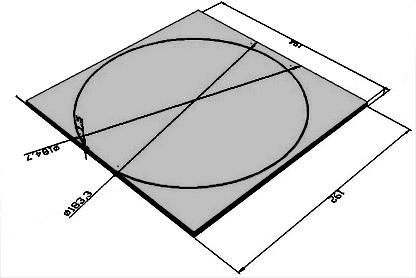
\includegraphics[width=0.3\linewidth]{images/hcal-cell-single-plastic-element.png}
    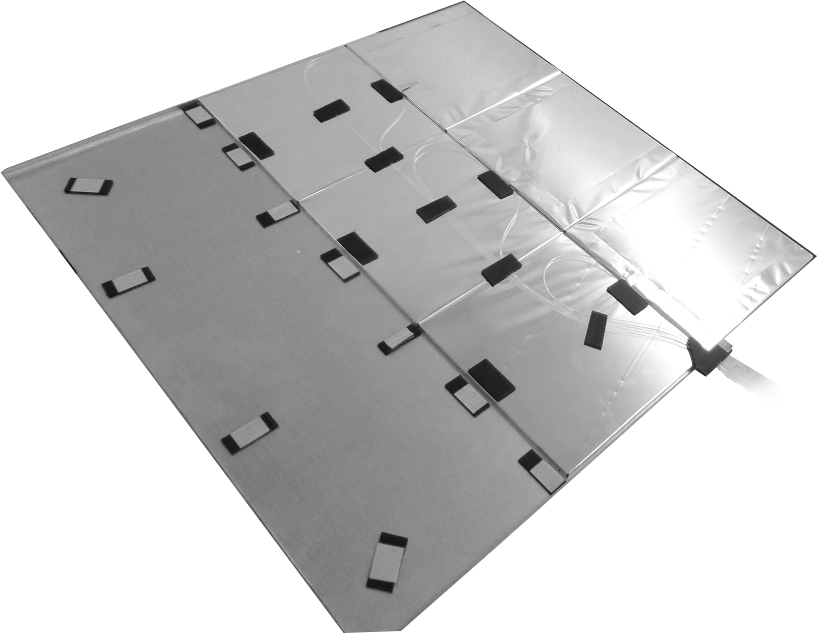
\includegraphics[width=0.3\linewidth]{images//illustrative/hcal-inlet-photo.png}
    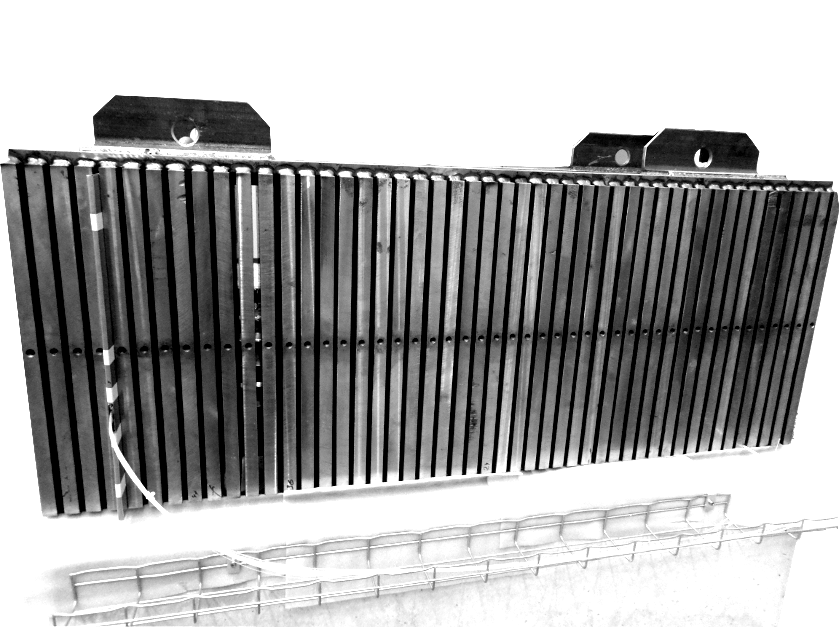
\includegraphics[width=0.3\linewidth]{images//illustrative/hcal-frame-photo.png}
    \caption{Схема укладки оптического волокна, фотографии вкладыша и сварного каркаса HCAL~\cite{PolyakovHCALDrawings-na64site}}
    \label{fig:hcal-module}
\end{figure}

Для задач калибровки калориметра важно, что \acrshort{mip} для
заряженных мюонов $\simeq1{,}55~\text{ГэВ}$ ($32{,}4~\text{МэВ}$ на слой)

Волокна от пластин отвечающих выделенному продольному направлению
соединяются на фотокатоде одного~\acrshort{pmt}, предоставляя
информацию об одной чувствительной пространственной <<ячейке>>
ориентированной вдоль пучка.

Детектор играет важнейшую роль в случаях, когда в электромагнитном
калориметре происходит адронизация компонент
ливня (<<адронный хвост>>) -- в
основном это реакции с выходом пионов: фотоядерные
реакции~$\gamma + Z \rightarrow \pi + Z$ (десятки мб на ядро Pb),
каскадные реакции оброзования т.н. leading
neutrals \cite{leading-neutron-hera} (нейтронов и каонов)
фотодезинтеграция ядер, фоторождение $\eta$-мезонов ($0{,}01$ мб),
адронизация через $\rho$-мезон и т.д. Интегральная вероятность
образования высокоэнергетических нейтральных адронов с энергией
от одного до $100~\text{ГэВ}$ составляет $10^{-9}-10^{-8}$
частиц на инициирующий электрон. Для статистики
свыше~$10^{12}$ играет значительную роль также нейтральная компонента
исходного пучка (т.н. адронное
загрязнение $\pi^0$, $K^0$, $\gamma$-кванты), обсуловленное
методами получения первичного пучка, которые также
идентифицируется HCAL опираясь на пространственные
характеристики ливня.

\subsection{Микроструктурные детекторы}

В качестве трековых детекторов высокого разрешения в NA64 применяются
детекторы GEM (Gas Electron Multiplier)~\cite{gems-sauli} и 
MicroMega (MICRO-MEsh GAseous Structure)~\cite{na64-BANERJEE201872}. Оба типа детекторов
относятся к семейству т.н. \emph{микроструктурных детекторов с газовым
усилением}. Общая идея регистрации заряженной частицы этими детекторами
состоит в регистрации электронной ионизационной лавины развивающийся
в газовой смеси при прохождении заряженной частицы планарной структурой
из тонких (десятки-сотни мкм) электродов.

Основное отличие GEM и MicroMega заключается в конструктивной реализации
принципа газового усиления. В детекторах GEM усиление реализуется за счёт
локального увеличения напряжённости вблизи отверстий перфорирующих тонкую
полимерную фольгу с металлизацией, на которую подаётся разность потенциалов.
Считывание затем производится с металлизированного катодного слоя на
стенке газового объёма, как изображено на рисунке~\ref{fig:gem-charge-collection}.
\begin{figure}
    \centering
    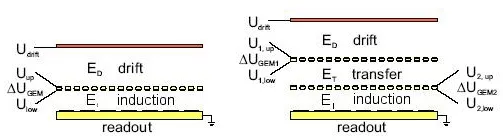
\includegraphics[width=0.65\linewidth]{images//illustrative/gem-charge-collection.png}
    \caption{Схематическое изображение гальванического усиления и зарядового
    считывание в объёме детектора GEM \cite{gems-compass}}
    \label{fig:gem-charge-collection}
\end{figure}
В детекторах MicroMegas, напротив, усиление происходит в узком газовом
зазоре между анодной платой и тонкой металлической сеткой, создающей
градиент электрического поля как показано на рисунке~\ref{fig:mumega-charge-collection}.
Таким образом, в GEM принцип газового
усиления реализуется каскадом электродов, а MicroMegas --
однородной областью лавинного умножения непосредственно над анодом.
\begin{figure}
    \centering
    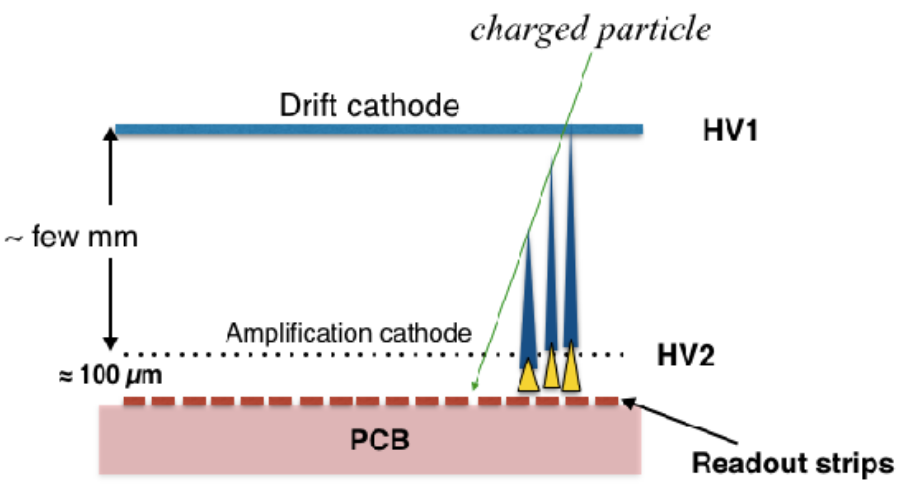
\includegraphics[width=0.65\linewidth]{images//illustrative/mm-charge-collection-example.png}
    \caption{Регистрация треков в рабочем объёме детектора MicroMega \cite{na64-BANERJEE201872}}
    \label{fig:mumega-charge-collection}
\end{figure}

В NA64 оба типа детекторов представлены в микростриповом исполнении --
анод выполнен в виде полос нанесённых литографическим методом на тонкую
подложку (каптон). Каждая такая плоскость даёт информацию
о координате вдоль одного направления. Для восстановления пространственной
точки попадания частицы в рабочий объём плоскости монтируются в виде
отдельных станций состоящих из двух плоскостей, дающих проекционную
информацию о месте развития электронной лавины вдоль пары перпендикулярных
координатных осей (годоскопический принцип).

%TODO: размеры
Рабочий объём детекторов продувается смесью $\text{Ar}/\text{CO}_2$ 80/20\%
при атмосферном давлении.

Считывание электрических сигналов осуществляется посредством
демультиплексирования амплитудных импульсов со всего массива полос на
плоскости и последующего преобразования амплитудного сигнала в цифровую форму.
За аналоговое демультиплексирование отвечает интегральная
микросхема APV~\cite{apv-jones},
в то время как сэмплирующее амплитудно-цифровое преобразование осуществляется
микросхемой MSADC.

Несмотря на хорошее координатное разрешение ($\simeq 300-400\text{мкм}$
при ширине анодной полоски $250~\text{мкм}$ для MicroMegas и $200~\text{мкм}$
при ширине $140~\text{мкм}$ для GEM) и
устойчивость отклика при высоких загрузках, микроструктурные
детекторы NA64 имеют ограниченную площадь чувствительной поверхности
($180\times180~\text{мм}$ для MicroMegas и $102{,}4\times102{,}4~\text{мм}$
для GEM) и применяются в основном в системе мечения.

\subsection{Детекторы на основе тонкостенных трубок}

Для увеличения аксептанса, трекер NA64 может быть оснащён станциями
состоящими из тонкостенных дрейфовых трубок~(\emph{straw})~\cite{straws-volkov2019, straws-peshekhonov2015}.
Каждая трубка представляет собой цилиндрическую поверхность выполненную
из гибкой полимерной плёнки с металлизацией (катода) с протянутой
вдоль её оси проволокой-анодом. Через массив трубок продувается
смесь $\text{Ar}/\text{CO}_2$ (80/20\%) при атмосферном давлении.

Принцип измерения координат основывается на регистрации времени дрейфа
ионизационных электронов к аноду отдельной трубки, как показано
на рисунке~\ref{fig:straws-measurement}.

\begin{figure}
    \centering
    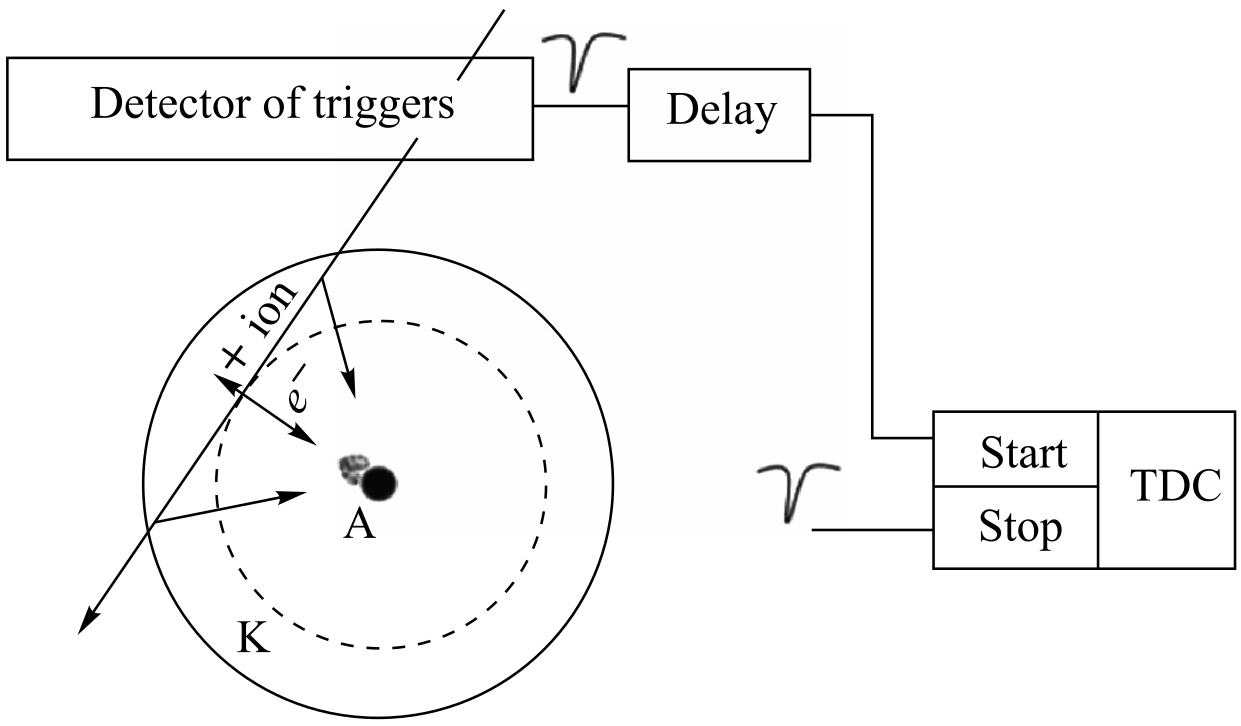
\includegraphics[width=0.5\linewidth]{images//illustrative/strawa-principle.png}
    \caption{Схема измерения времени дрейфа ионизационных электронов~\cite{straws-peshekhonov2015}}
    \label{fig:straws-measurement}
\end{figure}

Для NA64 были изготовлены станции трёх типов:
\begin{itemize}
    \item $200\times200~\text{мм}$ С внутренним диаметром
    трубок $6{,}02 \pm 0{,}025~\text{мм}$, и толщиной
    стенки~$62~\text{мкм}$, с металлизацией алюминием толщиной $500~\mathring{\text{A}}$.
    В качестве анода используется позолоченная вольфрамовая проволока диаметром $30~\text{мкм}$.
    \item $200\times200~\text{мм}$ С внутренним диаметром
    трубок $2 \pm 0{,}025~\text{мм}$, и толщиной
    стенки~$67~\text{мкм}$, с металлизацией алюминием толщиной $200~\text{нм}$
    и дополнительным покрытием защитным слоем графитополиуретана толщиной~$6~\text{мкм}$.
    В качестве анода используется позолоченная вольфрамовая проволока диаметром
    $20~\text{мкм}$.
\end{itemize}

С точки зрения трекинга, измеренное время сигнала $t$ с анода задаёт
изохронную цилиндрическую поверхность с радиусом $r = t v$, где
$v$ -- характерная скорость дрейфа электронов в газовой смеси.
Алгоритмически, такие изохронные поверхности способны приводить к
неоднозначностям при реконструкции трека, поэтому станции обычно состоят
из массивов тонкостенных дрейфовых трубок или являются частью
многоступенчатого трекера.

\subsection{Номенклатура детекторов}

С целью охвата всей номенклатуры детекторов в рамках программных
моделей имеющих дело с данными эксперимента в общем (и с моделью
события в частности), необходимо учесть следующие обстоятельства,
связанные с представлением данных на низком уровне 

На уровне отдельных измерений, состав (тип и топология)
данных полностью определяется основной микросхемой (\emph{чипом})
считывающего электронного устройства, осуществляющего
преобразование аналоговых сигналов.
Это означает, в частности, что сигналы оцифрованные с калориметра,
пучкового счётчика, вето-детектора и мюонного счётчика будут
содержать одну и ту же информацию в смысле типа данных, поскольку
считываются одним и тем же чипом. В то же
время, сигнал от микроструктурных детекторов --- будь
то GEM или MicroMega будут иметь другой тип данных.

Таким образом, с точки зрения физического представления данных,
целесообразно поместить показания от одного чипа в
гомогенную коллекцию. Тогда статический
\gls{allocator} коллекции будет иметь дело
с данными одного типа, что уменьшит фрагментацию данных и
улучшит локальность кэширования. Дополнительным преимуществом
такого решения является возможность итерировать всю такую коллекцию
в рамках одной лексемы -- во многих случаях прикладные алгоритмы
(обработчики конвейера данных) нуждаются в доступе такого вида.
Например, алгоритм вычисления сигнала нулевого уровня
совершенно агностичен к тому, к какой станции,
или к какому типу детекторов относится оцифрованный сигнал.

Следующим важным элементом классификации детекторов является деление
по \emph{семействам} (англ. \emph{kin}), для которых в системе
сбора данных NA64 приняты обозначения подобные приведенным в
таблице \ref{tab:detector-names-examples}.

\begin{table}[ht]
\centering
\begin{tabular}{r|cl}
Наименование & Чип     & Описание \\ \hline
          S1 & MSADC   & Первый пучковый счётчик \\
        VETO & MSADC   & Вето-детектор \\
        ECAL & MSADC   & Электромагнитный калориметр \\
        GM03 & APV     & Газовый электронный умножитель №3 \\
        MM02 & APV     & Микросеточный газовый детектор №2  \\
        ST06 & NA64TDC & Трубчатый дрейфовый детектор №6
\end{tabular}
\caption{Примеры имён детекторов}
\label{tab:detector-names-examples}
\end{table}

Наконец, необходимо индексировать отдельные чувствительные
элементы детектора. В зависимости от семейства к которому принадлежит
детектор, это могут быть ячейки калориметра, проекционные
плоскости трековых детекторов, трубки газовых детекторов.

В результате, дескриптор уникально идентифицирующий чувствительный
элемент детектора должен отражать следующую семантику (в порядке
убывания общности):

\begin{enumerate}
    \item Идентификатор типа микросхемы (чипа, <<chip>>), определяющий
    тип данных,
    \item Идентификатор семейства детектора (<<kin>>), дающий информацию о
    физическом смысле сигнала,
    \item Номер станции, для уникальной идентификации детектора в
    пределах одного семейства,
    \item Нагрузку (<<payload>>), содержащую информацию о конкретном
    чувствительном элементе детектора, в зависимости от чипа или семейства.
\end{enumerate}

Для калориметров и сегментированных детекторов с \acrshort{pmt},
нагрузке достаточно содержать три индекса, идентифицируюших
ячейку или сегмент детектора.

Для микроструктурных трековых детекторов нагрузка должна содержать
информацию об ориентации проекционной плоскости детектора и номер
чувствительного элемента.

Простой расчёт показывает, что всю номенклатуру детекторов NA64
можно уместить в множестве мощностью не более $2^{64}$ значений,
что позволяет, в принципе, использовать номерной идентификатор
для кодирования дескриптора детектора. Это в свою очередь позволяет свести
операции запроса и поиска элементов коллекций до простых
операций с целым числом фиксированной длины, осуществлять выборку
элементов применением быстрых побитовых операций и т.д.


\begin{comment}
\subsection{Моделирование э/м ливня}

Для оценки вклада в разрешения факторов обусловленных физикой ливня
воспользуемся эмпирической формулой разрешения для слоистого калориметра с
заданной геометрией~\cite{delPeso1989-sampling-calorimeters}:
\begin{equation}
    \frac{\sigma_{sampl}}{E}(\%) = \frac{3.5}{\sqrt{E}}
        \cdot \left( \frac{t}{X_t} \right)^{\alpha}
        \cdot \left( \frac{s}{X_s} \right)^{\beta},
\end{equation}
где $t, X_t, s X_s$ --- толщина и радиационная длина слоёв сцинтиллятора и
свинца, соответственно, а $\alpha, \beta$ --- некоторые подстроечные  % e.g. alpha=0.67, beta=-0.3
коэффициенты, которые обычно определяются из МК-модели
калориметра (в оригинальной работе~\cite{delPeso1989-sampling-calorimeters}
моделирование производилось в пакете EGS4, 1988). % TODO использующего модели
Современный (напр. 4.10.6) Geant4 предоставляет возможность использовать
различные комбинации моделей процессов электромагнитного ливня с тем чтобы
обеспечить наилучшее согласие в известном диапазоне энергий.

Для моделирования развития ливня зададим геометрию калориметра в виде цилиндра
составленного из круговых пластин сцинтиллятора и свинца с толщинами
соответствующих слоёв ECAL. Получившуюся модель цилиндрического калориметра
сегментируем по $\rho, \phi, z$ с тем чтобы для заданной энергии инициирующей
частицы получить \emph{энергетический профиль} э/м ливня в виде функции со
следующей факторизацией:

\begin{equation}
    \dd E(\rho, z) = E/2\pi \cdot f(\rho) \dd \rho \cdot f(z) \dd z.
    \label{eq:emshowerFac}
\end{equation}

Нужно заметить, что факторизация \eqref{eq:emshowerFac} справедлива только для
перпендикулярного направления движения частицы по отношению к пластинам
калориметра. В силу анизотропии размещения поглотителя в веществе калориметра,
такая факторизация перестаёт работать.
% ^^^ интересным приложением может быть реконструкция угла падения частицы на
% основе такой информации --- хотя вклад от \phi по-видимому нельзя
% факторизовать, вероятно возможно подобрать декомпозицию другого рода...

\subsection{Продольный профиль э/м ливня}

Известно, что продольный профиль ливня хорошо описывается
$\Gamma$-распределением \cite{Longo1975EMCSim}:

\begin{equation}
    \left\langle \frac{1}{E} \frac{\dd E(z)}{\dd z} \right\rangle = f(z) = \frac{(\beta z)^{\alpha-1} \beta \exp(-\beta t)}{\Gamma (\alpha)},
\end{equation}
где $\alpha$ регулирует форму продольного профиля а $\beta$ --- масштаб.  %< TODO: "масштаб"?
Центр масс $\langle z \rangle$ энергетического распределения связан с этими
параметрами как $\langle z \rangle = \alpha / \beta$, а максимум может быть
выражен как $\max f(z) = (\alpha - 1)/\beta$.
\end{comment}
\section{Аналого-цифровые преобразователи}

%В NA64 для оцифровки сигнала с \acrshort{pmt} счётчиков, вето-детекторов и
%калориметров применяются аналого-цифровые преобразователи MSADC \cite{MSADC-Mann1, %MSADC-Mann2} (\emph{англ} Mezzanine sampling analog to digital converted).
Для оцифровки сигналов формируемых \acrshort{pmt} (пучковых счётчиков,
вето-детекторов и калориметров) в NA64 применяются
аналого-цифровые преобразователи MSADC \cite{MSADC-Mann1, MSADC-Mann2}
(англ. \emph{Mezzanine Sampling Analog-to-Digital Converter}).
MSADC представляет собой устройство на основе микросхемы
ADS527x~\cite{ADS527x}, выполненное в виде мезонинной карты расширения
в стандарте <<Advanced Telecom Computing Architecture>> (ATCA).
Конструктивно, предусмотрен монтаж устройства как в
корзину (крейт) системы сбора данных, так и в непосредственной близи
детекторной сборки для уменьшения длин аналоговых линий и уменьшения помех.
MSADC в установке NA64 применяются как для непосредственного считывания
сигналов \acrshort{pmt}, так и опосредованно, для оцифровки сигналов
от микропаттерных детекторов предварительно подаваемых на вход
аналогового демультиплексора.

В рамках первого сценария каждый аналоговый канал считывается двумя сэмплирующими
АЦП, работающими на частоте $40\text{МГц}$. Каналы тактируются со
смещением в половину
фазы, обеспечивая сэмплирование сигнала с интервалом 12.5нс (с
частотой~$80\text{МГц}$). На рисунке \ref{fig:msadc-example} приведён
характерный пример гистограммы полученной на основе $8\times10^3$ событий в
центральной ячейке калориметра ECAL, с отбором по пучковому триггеру.

\begin{figure}
    \centering
    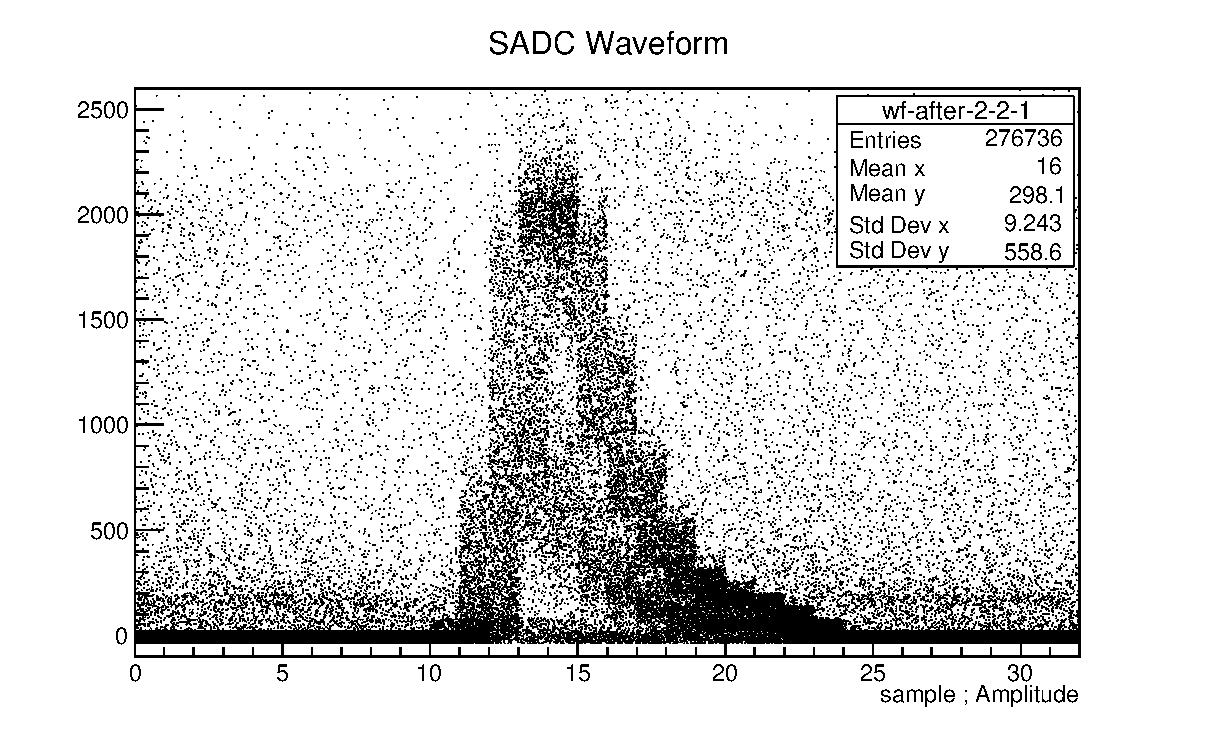
\includegraphics[width=0.65\linewidth]{images/illustrative/msadc-waveforms-example.eps}
    \caption{Гистограмма характеризующая временную развёртку амплитудного сигнала в
    центральной ячейке от моноэнергетического пучка}
    \label{fig:msadc-example}
\end{figure}

Для регистрации сигнала от сцинтилляционных детекторов в эксперименте
применяются ФЭУ-84~\cite{soviet_pmts}, для которых время нарастания
импульса анодного тока не превышает одной наносекунды. При этом
характерная длительность (ширина на половине амплитуды) импульсов от
большинства детекторов лежит в диапазоне от двух до трёх наносекунд.

Следует отметить, что согласно теореме Котельникова (Найквиста-Шеннона),
для безошибочного восстановления сигнала с таким характерным временем,
необходима частота дискретизации не менее $800\text{МГц}$ (частота
Найквиста для сигналов длительностью $2{,}4\text{нс}$).

С целью разрешения единичных импульсов от ФЭУ-84 в основном применяемых в
эксперименте, сигнал от \acrshort{pmt} передаётся сначала на вход
предварительного преобразователя (шейпера выполненого на основе
операционного усилителя AD8021~\cite{ad8021}), увеличивающего характерную
ширину сигнала примерно в три раза с сохранением амплитудной
пропорциональности. Несмотря
на то что частоты $80\text{МГц}$ всё ещё недостаточно для безошибочного
разрешения сигналов с полушириной в диапазоне от $6$ до $9~\text{нс}$
(частота Найквиста составляет примерно $170\text{МГц}$), необходимой
точности восстановления временных характеристик сигналов можно
добиться используя априорную информацию о форме сигнала -- то есть,
подобрав аналитическую модель достаточно хорошо воспроизводящую сигнал,
способную восполнить недостающую информацию в частотном домене.

\subsection{Параметризация сигнала АЦП}

С целью определения основных свойств сигнала и выбора оптимальных моделей для
математической подгонки (фита), для различных детекторов была выполнена серия
измерений формы импульса до и после шейпера с применением цифрового
осциллографа с пикосекундным разрешением.

%При рассмотрении малых амплитуд (менее $100~\text{мВ}$) определённую
%практическую трудность создают различные помехи, обусловленные индуктивными
%эффектами при работе на высоких частотах, такие как эффекты индуктивных
%задержек и отражений в коаксиальных проводниках, неидельность волнового
%сопротивления во цепи между шейпером и осциллографом или \acrshort{pmt} или
%осциллографом. С целью снижения этих эффектов при проверке модели
%параметризации, для проверки модели параметризации в области малых
%амплитуд, было выполнено численное моделирование шейпера на основе его
%принципиальной схемы.
Анализ сигналов малой амплитуды (менее $100~\text{мВ}$) имеет
определённые практические трудности, обусловленные влиянием помех,
связанных с индуктивными эффектами, проявляющимися при работе на высоких
частотах. К числу таких эффектов относятся индуктивные задержки и
отражения в коаксиальных линиях передачи, а также отклонения
волнового сопротивления от номинального в линии связи между
шейпером и осциллографом и между шейпером и \acrshort{pmt}.

Для уменьшения влияния указанных факторов при проверке работоспособности
модели параметризации в области малых амплитуд было выполнено численное
моделирование работы шейпера на основе его принципиальной электрической
схемы в программном пакете LTspice~\cite{ltspice}.

%На рисунке~\ref{fig:ltspice-shaper-simulation} показан пример временной
%развёртки сигнала. Импульсам с отрицательной амплитудой соответствуют
%запись входного сигнала выполненного осциллографом с интервалом
%200 пикосекунд. Импульс с положительной амплитудой отображает результат
%симуляции.

На рисунке~\ref{fig:ltspice-shaper-simulation} приведён пример временной
развёртки сигнала. Импульсы с отрицательной амплитудой соответствуют
результатам регистрации входного сигнала осциллографом с временным шагом
дискретизации 2~пс, тогда как импульс с положительной амплитудой
представляет собой результат компьютерного моделирования.

\begin{figure}
    \centering
    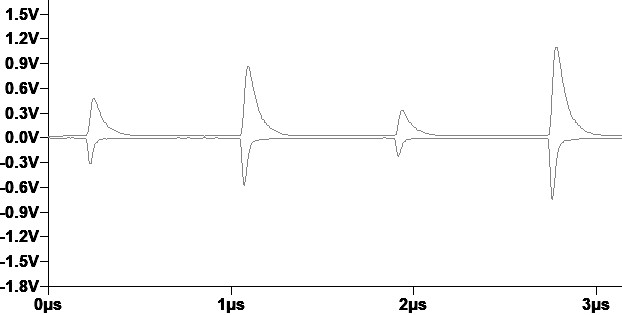
\includegraphics[width=0.75\linewidth]{images//illustrative/shaper-simulation.png}
    \caption{Результат моделирования преобразования сигнала в LTspice}
    \label{fig:ltspice-shaper-simulation}
\end{figure}

Моделирование достаточно хорошо (в пределах 1\%) согласуется с измеренным
выходным сигналом с амплитудами не менее нескольких десятков мВ.
На основании записанного сигнала в области больших
амплитуд, и с использованием численной модели LTspice, производилась проверка многопараметрических аналитических функций, способных воспроизводить форму
сигнала до или после шейпера.

%Количественные критерий, в виду сложной зависимости функции отклика от
%парамтров измерения, были сформулированы на основе важнейших физических
%параметров, а не общего численного соответствия. В частности, не
%рассматривалась точность поведения экспоненциального спадания импульса
%на интервалах превышающих ширину на полувысоте более чем вдвое, поскольку,
%в силу схемотехнических причин, последняя на этом участке слишком сильно
%зависит от парамтров шейпера имеющих большой разброс. Напротив, важными
%параметрами являлись:
Количественные критерии, учитывая сложную зависимость функции отклика
от параметров измерений, были определены на основе ключевых физических
характеристик, и в меньшей степени -- на основе общего численного
совпадения формы сигнала.
При этом не рассматривалась точность аппроксимации экспоненциального
спада импульса на временных интервалах, превышающих удвоенную ширину
на полувысоте, поскольку в данной области форма импульса существенно
зависит от параметров шейпера, характеризующихся значительным
технологическим разбросом.

В качестве основных критериев были выбраны:
\begin{itemize}
    \item Точка на переднем фронте импульса, соответствующая полувысоте
    импульса, принятая в качестве инвариантной временной метки (постоянная
    доля, англ. \emph{constant fraction}),
    \item Амплитуда в абсолютном максимуме импульса, как величина
    пропорциональная энерговыделению.
\end{itemize}

Помимо количественного соответствия сигналам, функции должны достаточно
просты для численного счёта, чтобы их можно было применять в различных
схемах нелинейной минимизации, таких как метод Ньютона, метод градиентного спуска
или алгоритм Левенберга-Марквардта~\cite{marquardt-lms}.

Итак, согласно выбранным критериям, рассматриваются следующие функции:

\begin{itemize}
    \item Функция Мояла \cite{moyalFunction} с тремя параметрами, определяемая выражением
    \begin{equation}
        F_M(t) = \frac{A}{\sqrt{2 \pi}} \exp \left\{ - \frac{1}{2} \left(\frac{x - \mu}{\sigma}+ \exp\left(\frac{x - \mu}{\sigma}\right)\right) \right\}
        \label{eq:moyalFNormed}
    \end{equation}
    которая адекватно описывает результат преобразования сигнала
    шейпером, позволяя использовать сравнительно простые аналитические формулы
    для временных характеристик (например, точки перегиба на переднем фронте) и амплитуды. Несмотря на присутствие быстро растущего множителя
    $e^{e^x}$, функция демонстрирует численную устойчивость при минимизации методом Левенберга–Марквардта с ускорением сходимости градиентом.
    \item Функция специального вида (N-pole), появляющаяся при различных
    аппроксимациях в некоторых статистических приложениях гамма-функции~\cite{gamma-stegun}:
    \begin{equation}
        f_{Np}\left(x\right)=A\left(x-t_{0}\right)^{n}e^{-\frac{\left(x-t_{0}\right)}{T}}\ \left\{x>t_{0}\right\}
    \end{equation}
    %хорошо описывает форму импульса до шейпера, воспроизводя быстрый рост
    %переднего фронта и обеспечивая устойчивые оценки
    %временных характеристик. При этом, аналитические выражения для времени
    %и амплитуды сигнала требуют вычисления специальных функций (гамма функции
    %и $W$ Ламберта). Из-за быстрого роста параметра $n$ функция требует
    %применения масштабных преобразований, иначе её сходимость нестабильна.
    %Также, при разрешении вкладов от близких по времени импульсов, функция
    %требует введения апостериорных ограничений для разрегения неоднозначности.
    которая хорошо воспроизводит форму импульса до шейпера, обеспечивая
    быстрое нарастание переднего фронта и стабильные оценки временных
    параметров. При этом аналитические выражения для времени и амплитуды
    сигнала требуют вычисления специальных функций --- гамма-функции и
    $W$-функции Ламберта. Из-за быстрого роста параметра $n$ функция
    требует применения масштабных преобразований для обеспечения
    сходимости численных алгоритмов. Кроме того, при разрешении
    наложенных импульсов с близкими по времени появлениями требуется
    введение апостериорных ограничений с целью устранения
    неоднозначностей.
    \item Четырёхпараметрическая функция из работы \cite{optimal-pulse-proc-samoyl}:
    \begin{equation}
        F(t) = A \cdot \exp(-(t-t_0)/\tau_1) /(1 + \exp(-(t-t_0)/\tau_2).
    \end{equation}
    %используется для аппроксимации импульсов с малой амплитудой. Практически,
    %независимость левого и правого фронтов приводят к необходимости
    %введения ограничений на основе апостериорных оценок.
    позволяющая независимо описывать участки нарастания и спада
    импульса. Эта функция применяется для аппроксимации сигналов
    малой амплитуды. Практически независимость параметров левого и
    правого фронтов требует введения апостериорных ограничений для
    обеспечения устойчивости.
\end{itemize}

%Применение описанных моделей позволяет описывать сигналы \acrshort{pmt}
%сэмплирующих АЦП в широком диапазоне энергий. В силу
%нелиности процедуры минимизации, наличия локальных
%минимумов, аппаратных шумов, а так же неоднозначности при разрешении
%вкладов от нескольких близких по времени частиц, практическое
%использование описанных параметризаций должно производиться в рамках
%программного окружения допускающего конкурентные сценарии,
%резервные алгоритмы условные ветвления и итеративную проверку гипотез.
Применение рассмотренных моделей позволяет адекватно описывать сигналы
\acrshort{pmt}, считываемые сэмплирующими АЦП в широком диапазоне энергий.
Ввиду нелинейности процедуры минимизации, наличия локальных минимумов
функции ошибки, а также влияния аппаратных шумов и неоднозначности при
разложении сигналов, формируемых несколькими близкорасположенными
во времени частицами, практическое использование данных параметризаций
должно осуществляться в программном обеспечении, обеспечивающем
поддержку конкурентных сценариев, резервных алгоритмов, условных
ветвлений и итеративной проверки гипотез.

\subsection{Уровень нулевого сигнала и эффекты высокой частоты}

%Уровнем нулевого сигнала (\emph{baseline}) называется значение оцифрованной
%амплитуды соответствующее отсутствию физического сигнала. Это значение
%обусловлено входным напряжением операционного усилителя во входном каскаде АЦП и
%балансировкой внутренних компараторов. Также, это значение определяется
%внутренними параметрами цепи и может быть подвержено
%незначительному дрейфу~($<1\%$), обусловленному изменениями гальванических
%характеристик линий преобразователя или изменением темнового тока \acrshort{pmt}
%под воздействием высокой интенсивности, термическими
%эффектами схемы, статистическими флуктуациями электронной лавины.
\emph{Уровнем нулевого сигнала} (\emph{baseline}) представляет собой значение оцифрованной амплитуды, соответствующее отсутствию сигнала на входе АЦП.
Формирование данного уровня обусловлено входным напряжением операционного
усилителя, используемого во входном каскаде АЦП, а также балансировкой
внутренних компараторов. Помимо этого, значение нулевого уровня определяется
внутренними параметрами входной цепи и может подвергаться незначительному
дрейфу (порядка $1 \%$ от уровня сигнала, что способно оказать заметное
влияние на разрешение некоторых детекторов), вызванному изменением
гальванических характеристик линий преобразователя, вариациями темнового
тока \acrshort{pmt} под воздействием высокой интенсивности, термическими эффектами
в электронной схеме, а также статистическими флуктуациями электронной
лавины.

Для повышения точности реконструкции энерговыделения в калориметре
необходимо применять устойчивый алгоритм выделения нулевого уровня, который бы
в наименьшей мере подвержен влиянию дрейфа и эффектам связанным с
интенсивностью пучка.

Существующий алгоритм динамического вычисления нулевого уровня заключается
в анализе первых нескольких сэмплов амплитудного сигнала и опирается на
предположение о том что в них отсутствует фактический сигнал. Последнее
обстоятельство гарантируется триггерной системой в смысле сигналов от
первичных частиц отслеживаемых триггерными счётчиками. Практически, нередки
события, когда сигнал в детекторе присутствует и обусловлен гало пучка, 
вторичными частицами и т.д. Если разброс
минимального и максимального значений превышает некоторый заданный порог,
за уровень нулевого сигнала берётся минимальное значение, в противном случае,
вычисляются средние. Результат работы такого алгоритма определяется
абсолютным порогом. На рисунке~\ref{fig:baselineresults} слева изображён
вариант работы такого алгоритма в случае, когда в окне оцифровки присутствует
остаточный сигнал от предыдущего события с амплитудой не превышающий
порог. Для наглядности, справа приведён результат работы улучшенного
алгоритма предложенного автором на основе минимизации невязок вторых
производных (\emph{деинтерлейсинг}), вместе с изображением результатов
аппроксимации модельными функциями.

\begin{figure}
    \centering
    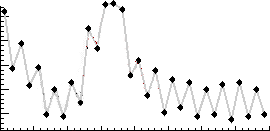
\includegraphics[width=0.33\linewidth]{images//illustrative/baselines-distorted.png}
    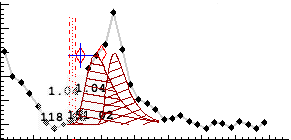
\includegraphics[width=0.33\linewidth]{images//illustrative/baselines-corrected.png}
    \caption{Отыскание нулевого уровня сигнала
    по первым сэмплам (слева) и на основе минимизации производных (справа)
    в относительных единицах}
    \label{fig:baselineresults}
\end{figure}

%В качестве иллюстрации, рассмотрим сигналы изображённые на рисунке ...

Появление отдельных событий на триггере установки определяется средней
интенсивностью пучка, и их число в любой конечный интервал времени является
случайной величиной, распределение которой соответствует закону
Пуассона~\cite{exp-methods-Abramov1977}.
Управляемая средняя частота триггерных событий
обычно выбирается таким образом чтобы влияние событий оказавшихся в пределах
одного временного окна считывания данных было не слишком велико (обычно
от 5 до 40\% в окне $400~\text{нс}$).

Идентификация таких событий имеет важное значение в первую очередь на этапе
калибровки, поскольку будет обуславливать систематическую ошибку средних
величин для заранее неизвестного энергетического вклада.

\iffalse
Руководствуясь первыми принципами возможно оценить статистический вклад от
таких событий с тем чтобы рассчитать соответствующие поправки, если известна
функция отклика от незашумлённых данных.

%Рассмотрим например детекторы, считывание данных с которых производится чипом
%MSADC (сэмплирующий АЦП) --- чип оцифровывает гальванический сигнал (обычно
%амплитудный испульс с \acrshort{pmt} после шейпера) в виде набора отдельных измерений с
%фиксированным интервалоом в пределах короткого временного окна. В качестве
%модельного приближения выберем далее функцию Мояла \cite{moyalFunction}:

%в которой, помимо положения максимума $\mu$ введём дополнительные параметры
%отвечающие за ширину и площадь ($\sigma$ и $S$):
%\begin{equation}
%    M(t, \vec{p}) = \frac{S}{\sqrt{2 \pi} \sigma} \exp\left\{ - \frac{1}{2} \left(\frac{t-\mu}{\sigma} + \exp\left(-\frac{t-\mu}{\sigma}\right)\right) \right\}.
%\label{eq:moyalF}
%\end{equation}

%Функцию \eqref{eq:moyalFNormed} обычно используют в качестве аналитической
%аппроксимации функции плотности распределения Ландау \cite{BockHEPFormulae}.

Задержка сигнальной линии относительно триггера выбирается таким
образом, чтобы разместить максимум импульса в середине сэмплирующего окна,
а для вычисления пьедесталов производится по первым нескольким каналам таким
образом, чтобы им соответствовал вероятный ноль сигнала.

\begin{figure}[h]
    \centering
    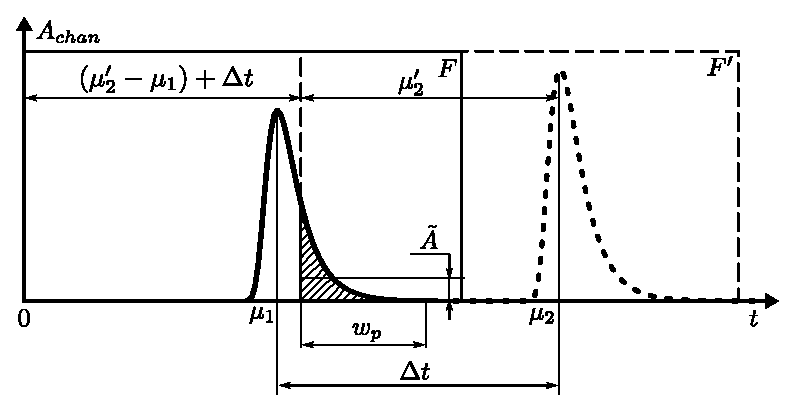
\includegraphics[scale=1.05]{pile-up-image-v2.eps}
    \caption{Схематическое изображение эффекта pile-up в амплитудно-временной
развёртке \acrshort{pmt}. Здесь, при оцифровке триггерного события (показано
пунктиром, вместе со своим окном дискретизации~$F'$) с максимальной
амплитудой в момент времени~$\mu_2 = \Delta t + \mu_2'$, в качестве значения
пьедестала будет взято среднее значение~$\tilde{A}$ на участке~$w_p$ которое
оказывается смещено относительно настоящего нуля за счёт вклада от события
$\mu_{1}$ (показано непрерывной линией вместе со своим окном дискретизации~$F$).}
    \label{fig:pileUpDiagram}
\end{figure}

Значение пьедестала $\tilde{A}$ определённое в окне
$w_p$, для каких-нибудь двух событий отклики которых заданы двумя наборами
параметров
$\mu_1, \sigma_1, S_1$ и $\mu_2, \sigma_2, S_2$, и произошедших с интервалом
$\Delta t$ можно записать в виде математического усреднения (см.
рис. \ref{fig:pileUpDiagram}):

\begin{equation}
\tilde{A} = \frac{1}{w_p} \int\limits_{\Delta t}^{\Delta t + w_p} (M(t, \mu_1, \sigma_1, S_1) + M(t, \mu_2, \sigma_2, S_2) \dd t
\end{equation}

Вклад $M(t, \mu_2, \sigma_2, S_2)$ будет ничтожным поскольку $w_p$ выбирается таким
образом, чтобы перекрыть участок до переднего фронта импульса триггерного
события, а дисперсия $\mu$ незначительна относительно ширины окна дискретизации
и $w_p$. Таким образом, модель можно редуцировать до плавающего окна усреднения
единственной функции $M(t, \mu_1, \sigma_1, S_1)$. Опустим индексы
для краткости, поскольку параметры триггерного события не влияют на результат: 

\begin{equation}
    \tilde{A}(\Delta t, \mu, \sigma, S) = \frac{1}{w_p} \int\limits_{0}^{w_p} M(t, \mu - \Delta t, \sigma, S) \dd t.
    \label{eq:avPedestal}
\end{equation}

Практический интерес представляет зависимость средней ошибки пьедестала от
средней частоты событий --- решение такой задачи даёт критерий для контроля
качества данных. Для того чтобы получить такую оценку аналитически, можно,
далее, взвесить и усреднить
функционал \eqref{eq:avPedestal} по $\Delta t$ и набору параметров
$\mu, \sigma, S$.


При этом, для правдоподобия модели критическое значение имеет
скоррелированность параметров $p_{n,(1)}$, --- в таком распределении
заключена основная информация о характере функции отклика единичного события.
Общий вид трёхмерной гистограммы распределения этих параметров показан на
рис. ???.
%TODO: 3D-гистограмма

Если каким-нибудь образом гарантировать отсутствие pile-up-событий в
гистограмме на рис. ???, то получившимся распределением можно воспользоваться
в качестве параметризации параметра модели.

Для частоты событий $\nu$ интервал между случайными событиями $\Delta t$
подчиняется экспоненциальному закону, таким образом среднее значение
пьедестала:

\begin{equation}
    \bar{A} (\nu) = \frac{\nu}{w_p} \int\limits_0^{\infty} \exp(- \Delta t \nu ) \left(
        \int\limits_{0}^{w_p} M(t, \mu - \Delta t, \sigma, S) \dd t \right) \dd \Delta t
\end{equation}
\fi

\section{Анализ данных}

Весьма важен вопрос анализа данных,
как процедуры обработки экспериментальных данных
направленной на проверку определённых статистических гипотез.
%В самом деле, процедуры сложно разделить
%практически, поскольку алгоритмы реконструкции содержат
%различные подстроечные параметры выбираемые из статистических
%соображений, с учётом физического процесса лежащего в основе
%конкретного измерительного процесса.

Сложившаяся практика работы с экспериментальными
данными обычно подразумевает разделение фаз отладки процедур
физической реконструкции событий и физического анализа данных.
У этого разделения есть как технические, так и методические причины.

К техническим относятся, например, многоэтапность процедуры
реконструкции, часто включающая применение итеративных операций,
использование алгоритмов с обратной связью. Кроме того,
%как уже отмечалось,
реконструкция в современном физическом эксперименте
как правило, представляет собой чрезвычайно требовательную задачу
к вычислительным ресурсам. По этой причине результат
реконструкции обычно сохраняется в виде промежуточных данных,
удобных для последующего анализа.

К методическим относится, например,
стратегии <<слепого анализа>>~\cite{blind-analysis} (анализа по слепому методу)
предписывающая экспериментатору исключать из рассмотрения
параметрические области, в которых может присутствовать исследуемый
сигнал до тех пор, пока все алгоритмы реконструкции и критерии отбора,
а также все процедуры анализа не окажутся
зафиксированы, и все проверки независимых данных, систематических
ошибок и методы статистической интерпретации результата не будут
выполнены.

Поскольку NA64 направлен прежде всего на поиск гипотетических частиц,
основная задача анализа сводится в вероятностном
смысле к проверке гипотезы $H_0$ о средней частоте событий с
заданным уровнем \emph{статистической значимости}~$\alpha$
(вероятность ложноположительного заключения).
В экспериментальной физике высоких энергий открытием считается
гипотеза подтверждённая на уровне статистической значимости
соответствующей $5\sigma$-квантилю нормального распределения,
что соответствует вероятности ложноположительного (ошибка первого рода)
результата~$\alpha =\text{erfc}(5\sigma) =2{,}866\cdot10^{-7}$.
%(вычисляемого как односторонний критерий нормального распределения).

В случае когда статистика сигнальных событий невелика, необходимо
учитывать эффекты связанные с дискретностью отдельных
событий (процесс Пуассона).

\begin{comment}
В частности, \eqref{eq:cls-definition} значит, что даже
в случае отсутствия ожидаемых фоновых событий в сигнальной
области~($\nu_b = 0$),
%$H_0$ на заданном уровне значимости принимается <<с допуском>>:
любая гипотеза предсказывающая число событий меньшее
$- \text{ln} ~\alpha$ будет отвергнута. Для некоторых
значений $\alpha$ минимальное
число событий приведено в таблице~\ref{tab:cls-alpha-examples}.
\begin{table}[ht]
    \centering
    \begin{tabular}{r|c}
        $\alpha$ & $s$ \\ \hline
        $0{,}1$ & $2{,}3$ \\
        $0{,}01$ & $4{,}6$ \\
        $1-\text{erfc}(5\sigma)$ & $15{,}0$
    \end{tabular}
    \caption{Минимальное число событий для различных $\alpha$}
    \label{tab:cls-alpha-examples}
\end{table}
\end{comment}

Допустим, нулевая гипотеза ($H_0$) состоит в том,
что частота событий равна $\nu_b$, а альтернативная
гипотеза $H_1$ заключается в том что $\nu > n_b$
(тест на избыточность).
Тогда в качестве критерия следует взять вероятность получить
такое же или большее число событий по сравнению с
наблюдаемым~$N$, для ожидаемого среднего~$\nu_b$:
%(односторонний доверительный интервал распределения Пуассона)
\begin{equation}
    P(n \ge N|\nu_b) = \sum\limits_{k=N}^{\infty} \frac{\nu_b^n e^{-\nu_b}}{n!}.
    \label{eq:poisson-no-bg}
\end{equation}

%Выражение \eqref{eq:poisson-no-bg} отвечает на вопрос <<какова вероятность
%получить число событий равное или большее $N$ при известной средней
%частоте $\nu_b$?>>. 
Если эта вероятность оказывается меньше заданного
уровня значимости $P(n \ge N|\nu_b) < \alpha$, гипотеза $H_0$ отвергается,
что можно качественно интерпретировать как то, что событий оказалось
<<слишком много>>, чтобы их можно было достоверно объяснить
только фоновыми событиями.

% Ошибка 1-ого рода: отвергнуть правильн. (её вер-ть -- alpha, "уровень значимости")
% Ошибка 2-ого рода: принять неправильн. (её вер-ть -- beta, "1-мощность")
%
%  решение \ истин. | true     | false
% ------------------+----------+--------
%   posit. (reject) | 1-\beta  | \alpha (1st err)
%   negat. (accept) | 1-\alpha | \beta (2nd err)
%

При этом ошибку второго рода -- %(принятие неправильной гипотезы)
неверное объяснение наблюдаемых событий фоновыми явлениями,
нужно рассматривать с учётом предположения о частоте
сигнала~$\nu_s$. Мощность критерия связана с вероятностью ошибки
второго рода $\beta(\nu_s)$ следующим образом:
\begin{equation}
    P(n \ge N|\nu_b + \nu_s)
        = 1 - \beta(\nu_s) = e^{-(\nu_b + \nu_s)} \sum\limits_{n=N}^{\infty} \frac{(\nu_b + \nu_s)^n}{n!}.
\end{equation}
тогда сравнение с уровнем статистической значимости 
будет ошибочно принимать $H_0$ для всех $\nu_s$ в случае
когда $P(n \ge N|\nu_b + \nu_s)\ge\alpha$. Таким образом, даже
в случае, когда фоновые события не ожидаются ($\nu_b = 0$),
и событий в эксперименте не наблюдалось вовсе ($N=0$),
любая гипотеза предсказывающая частоту $\nu_s > -\text{ln}(\alpha)$
будет отвергнута. Этот на первый взгляд тривиальный результат
существенно важен для
выводов о чувствительности эксперимента, поскольку позволяет
в определённом доверительном пределе (англ. \emph{confidence limit},
$\text{CL}_{s+b} = P(n \ge N|\nu_b + \nu_s)$)
исключить область параметрического пространства на основе
набранной статистики. Таблица \ref{tab:cls-alpha-examples}
содержит значения $\nu_s$ для некоторых доверительных пределов часто
используемых в литературе.

\begin{table}[ht]
    \centering
    \begin{tabular}{r|c}
        $\text{CL}_{s+b} = 1 - \alpha$ & $\nu_s$ \\ \hline
        $0{,}9$ & $2{,}3$ \\
        $0{,}99$ & $4{,}6$ \\
        <<$5 \sigma$>>, $ 1 - \Phi(5)$ & $15{,}0$
    \end{tabular}
    \caption{Максимальное число событий принятия $H_0$ для
    различных значений доверительного предела при отсутствии
    фона}
    \label{tab:cls-alpha-examples}
\end{table}

В формулировке условной вероятности,
%\footnote{Условная вероятность $P(A|B) = P(A \cap B) / P(B)$.}
%включающей предположение о частоте сигнала $\nu_s$.
вероятность $\epsilon$ наблюдать $N$ или менее событий из
которых $N$ или менее событий составляют фоновые, при уровне
сигнала~$\nu_s$~\cite{cls-mtd-zech}:
\begin{equation}
    \epsilon =P(n \le N | n_b \le N, \nu_s + \nu_b) = \frac{P(n \le N | \nu_s +\nu_b)}{P(n_b \le N | \nu_b)}.
    \label{eq:cls-cond-prob}
\end{equation}

Следует заметить, что формулу~\eqref{eq:cls-cond-prob} можно
интерпретировать по-разному. Полученная первоначально из
байесовского подхода, она получила применение в
экспериментальной физики частиц и в рамках частотной
интерпретации, обобщённая в
т.н. $\text{CL}_s$-метод~\cite{cls-harel, read-cls} --- консервативный
способ установить верхний предел на сигнал в условиях малой
чувствительности эксперимента. Общая идея метода состоит в
определения отношения вероятностей под гипотезами <<сигнал+фон>>
и <<только фон>>, как записано в~\eqref{eq:cls-cond-prob},
однако направление интегрирования (для счётных статистик -- суммирования)
обычно обращают. Вводя параметр $\mu$ как величину определяющую вклад сигнала
(англ. \emph{signal strength}) в полную частоту
событий $\mu \nu_s + \nu_b$, записывают:
\begin{equation}
    \text{CL}_s (\mu) = \frac{\text{CL}_{s+b}}{1 - \text{CL}_b} = \frac{P(n \ge N | \mu\nu_s + \nu_b)}{P(n \ge N | \nu_b)}.
    \label{eq:cls-definition}
\end{equation}

%Для правильного понимания формулы \eqref{eq:cls-definition} важно
%иметь в виду, что $\text{CL}_x$ -- символическая запись,
%и $CL_{x} \ne P(x)$. В частности, $\text{CL}_s$ вообще не имеет
%вероятностного смысла.

Вклад сигнала $\mu$ считается исключённым со статистической
значимостью $\alpha$ в критической области $\text{CL}_s(\mu) < \alpha$.

%Важно отметить, что принятие гипотезы $H_0$ (отсутствие сигнала)
%на заданном уровне статистической значимости, не исключает
%гипотезу $H_1$. Принятие $H_0$ значит, что чувствительности
%эксперимента оказалось недостаточно для того, чтобы обнаружить
%статистически-значимый сигнал. По этой причине в поисковых
%исследованиях большое значение имеет указание параметрической
%области (и соответствующего порога статистической значимости)
%в которой сигнал не был обнаружен.

%We define CLs+b the "confidence level" as the probability to
%observe a number of events
%larger than the one observed in the experiment

%\begin{equation}
%    \text{CL}_{s+b}
%        = e^{-(\nu_s + \nu_b)}\sum\limits_{n=0}^N
%          \frac{(\nu_s + \nu_b)^n}{n!}
%\end{equation}

%Следует заметить, что такое упрощённое рассмотрение пренебрегает
%ошибкой при определении частоты фоновых событий и не учитывает
%влияние систематических ошибок.
%Современный статистический аппарат
С целью учёта систематических ошибок этот подход развивают,
в рамках односторонней статистики функций
правдоподобия $L(\mu, \theta)$ с \emph{мешающими параметрами} $\theta$,
%где $\mu$ регулирует вклад сигнала в частоту наблюдаемых
%событий $\mu \cdot \nu_s +\nu_b$
обобщая $\text{CL}_s$, и рассматривая теперь вместо статистики счёта
пуассоновских процессов статистику
профильного отношения
правдоподобия $q_\mu$~\cite{bityukov-krasnikov, read-cls, cls-harel}.
%Пусть регистрируемое число событий $\mu \cdot \nu_s + \nu_b$, где
%$\mu \in [0,1]$. Тогда функция правдоподобия записывается
% как вероятность одновременна вероятность иметь ... отнесённая к ...
\begin{equation}
    q_{\mu} = -2 ~\text{ln} \frac{L(\mu,\hat{\hat{\theta}})}{L(\hat{\mu}, \hat{\theta})}.
    \label{eq:qm-stat}
\end{equation}
Тогда ограничение на $\mu$ выводится из условия $\text{CL}_s (\mu) < \alpha$, где:
\begin{equation}
    \text{CL}_s = \frac{P_{s+b} (q_\mu \ge q^{obs}_{\mu})}{P_{b} (q_\mu \ge q^{obs}_{\mu})}
\end{equation}

Практически, рассматривая пространство из $m$ измеряемых величин,
часто используют гистограмму в качестве основной структуры данных
представляющих результаты измерения. В этом случае, функция
правдоподобия определяется как частотная вероятность в каждом
счётчике $j$ гистограммы:
\begin{equation}
    L(\mu,\theta) =\prod\limits_{j} \frac{\mu s_j + b_j}{n_j!}
        \prod\limits_{l} \prod\limits_{k} \frac{u_k^{m_k} (\theta_l)}{m_k!} e^{-u_k (\theta)}.
\end{equation}
%Если  $$ Функции правдоподобия $L(\mu, \theta)$ определяются 

Максимизация \eqref{eq:qm-stat} в малой окрестности $\theta_l$ позволяет
оценивать верхнюю границу доверительного интервала.

Метод $\text{CL}_s$ широко применяется в экспериментальной физике
высоких энергий для получения эффективного верхнего предела на сигнал,
с учётом перенормировки статистической значимости на фоновые события
и эффективность детектирующей аппаратуры.


\begin{comment}
%  решение \ истин. | true     | false
% ------------------+----------+--------
%   posit. (reject) | 1-\beta  | \alpha (1st err)
%   negat. (accept) | 1-\alpha | \beta (2nd err)
\begin{table}[ht]
    \centering
    \begin{tabular}{r|cc}
  Решение теста & $H_0$ верна     & $H_0$ не верна \\ \hline
   posit. (reject $H_0$) & FP, I-ого рода $P=\alpha$ & TP, $P=1-\beta$ \\
   negat. (accept $H_0$) & TN, $P=1-\alpha$ & FN, $P=\beta$ (II-ого рода) \\
    \end{tabular}
    \caption{Соответствие терминов ($\alpha$ -- стат. значимость, иначе <<доля FP среди случаев когда $H_0$ верна>>, вероятность отвергнуть правильную гипотезу;
    $\beta$ -- мощность критерия, вероятность того что нулевая гипотеза отвергнута, если верна конкурирующая)}
    \label{tab:placeholder}
\end{table}

В случае присутствия фонового вклада
часто прибегают к методу $CL_s$~\cite{cls-mtd-zech, read-cls}
представляющий собой консервативный способ выставления
верхних ограничений на сигнал.

Вероятность процесса Пуассона со средней частотой
$\nu_s + \nu_b$ даётся произведением вероятностей двух независимых
процессов в сумме дающих все возможные комбинации $n = n_s +n_b$:
\begin{equation}
    p(n;\nu_s+\nu_b)
      = \sum\limits_{n_b=0}^{n} \sum\limits_{n_s = 0}^{n-n_b}
            p(n_b;\nu_b) \cdot p(n_s;\nu_s)
      = \frac{1}{n!} (\nu_s+\nu_b)^n e^{-(\nu_s+\nu_b)}.
    \label{eq:frequentist-sb}
\end{equation}

Это выражение непригодно для непосредственных вычислений с
малыми~$n$, поскольку может приводить к отрицательным
значениям~$P$ в силу дискретности распределения
Пуассона~(в случае когда $b$ достаточно велико).
Последнее обстоятельство нужно учесть в первой
сумме~\ref{eq:frequentist-sb} имея в виду, что $n_b \ge N$.

Тогда вероятность $\epsilon$ наблюдать $N$ или менее
событий из которых $N$ или менее событий составляют фоновые,
при уровне сигнала~$\nu_s$:
\begin{equation}
    \epsilon
    = \frac{\sum\limits_{n=0}^N p(n;\nu_s+\nu_b)}{\sum\limits_{n_b=0}^N p(n_b;\nu_b)}.
    \label{eq:zach-prob}
\end{equation}

Выражение \eqref{eq:zach-prob} имеет смысл условной вероятности.
В общем случае, справедливо, что
\begin{equation}
    P(n \le N | n_b \le N, \nu_s + \nu_b) = \frac{P(n \le N | \nu_s +\nu_b)}{P(n_b \le N | \nu_b)}.
    \label{eq:cls-cond-prob}
\end{equation}

Это выражение можно использовать для вычисления доверительного
интервала в ситуациях анализа параметрических областей с фоном.
В литературе часто встречается альтернативная запись~\cite{cls-harel}:
\begin{equation}
    CL_s = \frac{p_{s+b}}{1 - p_b}
         = \frac{P(n \ge N | \nu_s + \nu_b)}{1 - P(n \ge N | \nu_b)},
\end{equation}
главное отличие которой от \eqref{eq:zach-prob} заключается
в направлении интегрирования (формулы эквивалентны).

Важно отметить, что принятие гипотезы $H_0$ (отсутствие сигнала)
на неком уровне статистической значимости, не исключает
гипотезу $H_1$. Принятие $H_0$ значит, что чувствительности
эксперимента оказалось недостаточно для того, чтобы обнаружить
статистически-значимый сигнал. По этой причине в поисковых
исследованиях большое значение имеет указание параметрической
области (и соответствующего порога статистической значимости)
в которой сигнал не был обнаружен.

Например, подстановка закона Пуассона в \eqref{eq:cls-cond-prob}
даёт $CL_s = e^{-\nu_s}$, что значит, что в случае
отсутствия событий в сигнальной области при известном (любом)
уровне фона, $H_0$ на заданном уровне значимости принимается
<<с допуском>>: любому заданному $\alpha$
отвечает максимальное число событий $- \text{ln} ~\alpha$ для которых
принята гипотеза $H_0$.
\begin{table}[ht]
    \centering
    \begin{tabular}{r|c}
        $\alpha$ & $s$ \\ \hline
        $0{,}9$ & $2{,}3$ \\
        $0{,}99$ & $4{,}6$ \\
        $\text{erfc}(5\sigma)$ & $15{,}0$
    \end{tabular}
    \caption{Значения $CL_s$ для различных $\alpha$}
    \label{tab:cls-alpha-examples}
\end{table}
Иными словами, на уровне значимости $\alpha$ гипотеза об отсутствии
сигнала не будет принята до тех пор, пока превышение сигнала над
уровнем фона не превосходит~$s$.

Более полное рассмотрение должно учитывать тот факт, что ожидаемый
фон в сигнальной области неоднороден. Как правило, случайная величина
характеризующая исследуемый феномен, заполняет гистограмму.

% ---

В этом случае рассматриваются
доверительные интервалы ($CL$) гипотезы о
частоте <<сигнал + фон>>~($CL_{s+b}$) и гипотезы о частоте
<<только фон>>~($CL_b$). Тогда консервативный критерий на
доверительный интервал гипотезы о сигнале при
заданном~$\alpha$ состоит в том что в параметрическом
пространстве сигнала должно выполнятся соотношение:
\begin{equation}
    CL_s = \frac{CL_{s+b}}{CL_b} < 1 - \alpha.
    \label{eq:cls-common}
\end{equation}

Необходимо заметить, что в то время как $CL_{s+b}$ и $CL_b$
являются интегралом функции плотности вероятности
(для распределения Пуассона -- отвечают $p$ в~\ref{eq:poisson-no-bg}),
запись $CL_s$ символическая, и имеет вероятностного смысла~\cite{cls-harel}.
Хотя подход исходит из частотной интерпретации вероятностей, стремясь
извлечь консервативную оценку для двух конкурирующих гипотез,
сам подход не является в полной мере ни частотным (поскольку рассматривает
ложноположительный исход), ни байесовским (поскольку не прибегает
к апостериорной оценке).

Удобно записать условие~\ref{eq:cls-common} в обозначениях условных
вероятностей:
\begin{equation}
    CL_s = \frac{P(q \ge q_{obs} | s+b)}{1 - P(q \ge q_{obs} | b)} \ge \alpha,
\end{equation}
где
\begin{itemize}
    \item $P(q \ge q_{obs}|s+b)$ -- вероятность получить такие же, или более
    экстремальные значения при условии <<сигнал+фон>>,
    \item $P(q \ge q_{obs} | b)$  -- вероятность получить такие же, или более
    экстремальные значения при условии <<только фон>>.
\end{itemize}
\end{comment}


\section{Функциональная организация}

На примере эксперимента NA64 хорошо прослеживаются общие черты
предметной области: экспериментальная установка организована
как комплекс автономных систем, синхронизируемых
посредством триггерного сигнала, эмерджентная задача которой состоит
в регистрации физических процессов, развивающихся в рамках
статистически независимых событий, с дальнейшими
вычислениями производимыми в рамках заданных доверительных
пределов.
%Отметим, что на этом (низком) уровне общности наиболее естественной
%формой представления данных является табличная модель.

По функциональному назначению (специализации) электромагнитный калориметр
совмещает роли мишени и детектора электромагнитных
ливней (т.н. активная мишень), участвуя в формировании триггерного
сигнала за счёт продольной сегментации. Трековые
детекторы предназначены для мечения (измерения энергии) отдельных
первичных частиц. Адронный калориметр завершает герметичность
установки, идентификацию процессов адронизации и измерение видимых
каналов. На этом уровне общности такие понятия как ливень
или траектория частицы удобно определять через группировку
отдельных низкоуровневых измерений в коллекции, дополняя
и доопределяя такие абстракции физическими величинами, по мере того
как от простых алгоритмов кластеризации и применения масштабных
преобразований уточняется и развивается информация о физике
процессов. В этом случае
%табличная модель перестаёт отвечать требованиям выразительности
%полноты информации,
в цифровом представлении физического события возникают
иерархические связи и конкурирующие гипотезы, что обуславливает
целесообразность использования объектной
модели события. При этом сам процесс удобно представлять в
форме изолированных инкрементных процедур,
в рамках конвейерного шаблона~--- посредством отдельных
обработчиков, обеспечивая гибкую и настраиваемую последовательность
реконструкции события.

При такой организации один и тот же обработчик
или участок конвейера может применяться и в рамках полного физического
анализа, и для отдельных тестов и калибровок, удовлетворяя нескольким
сценариям использования.

Возникает ряд прикладных задач допускающих обобщение:
\begin{itemize}
    \item Сравнение конкурирующих гипотез в рамках задач
    реконструкции треков и разделения
    сигналов \acrshort{sadc} представимо в формализме
    машин конечных состояний.
    \item Необходимость формулировать условия отбора событий
    и элементов его объектной модели (зарядовых кластеров,
    треков частиц, ливней, отдельных сигналов) представляет
    собой задачу достаточно часто включённую в другие, что
    обуславливает целесообразность специализированных выразительных
    средств для задания логических условий и арифметических операций.
    \item Другим примером частой потребности в отдельных
    алгоритмах обработки являются калибровочные данные
    представимые в виде текстовых таблиц.
    Реализация шаблона проектирования <<издатель--подписчик>>
    может быть дополнена специализированным выразительным
    средством с целью упрощения работы с такими артефактами.
    \item Единообразие номенклатуры данных и детекторов
    NA64 допускает принципиальную возможность хранения
    массива событий для последующей обработки.
    \item Очевидно, достаточно частой задаче в процедурах
    калибровки и отладки алгоритмов реконструкции
    является извлечение интегральных характеристик для элементов на
    определённом логическом уровне детекторов
    (ячейки, модуля калориметра, станции). Целесообразно предусмотреть
    автоматизированное средство для каталогизации таких объектов.
\end{itemize}

В то же время из содержания главы видны задачи являющиеся
в большой мере уникальными для NA64:
\begin{itemize}
    \item Кластеризация откликов координатных детекторов
    MicroMega, GEM и Straw,
    \item Вычисление радиуса цилиндрической изохронной поверхности
    для сигналов от тонкостенных трубок,
    \item Определение времени и энерговыделения в детекторах
    считываемых \acrshort{sadc},
    \item Калибровки ECAL, HCAL, VETO.
\end{itemize}

Существенный вклад в интерпретацию результатов экспериментальных
измерений вносят количественные оценки полученные с применением различных
методов моделирования. В частности, используется генератор
событий, реализующий модели аналитических сечений. Хотя сам по себе
такой генератор является достаточно изолированным низкоуровневым решением, его
использование в составе более обширной программной инфраструктуры
позволяет получить представление о картине исследуемого физического
процесса и чувствительности всей системы в целом.

Метод регистрации редких событий заключается в поверке
установки на известных и хорошо определённых процессах с известной
или проверяемой светимостью~--- <<стандартных свечах>>. Для NA64
определено несколько процессов в которых присутствуют такие сигналы.
Например, сравнительно частый ($\simeq10^{-4}$) процесс рождения и
выхода мюонных пар $\gamma\rightarrow\mu^{+}\mu^{-}$, или
более редкие процессы адронизации электромагнитного
ливня (фотоядерные реакции, $\simeq 10^{-8}$).

С методической точки зрения процедуры обработки реальных
экспериментальных данных и данных моделирования должны отличаться
лишь источником, то есть обработке результатов моделирования
отвечает всё тот же сценарий анализа.

Установка обеспечивает физические условия для поиска сигнальных
процессов и их регистрацию, а программное
обеспечение~--- воспроизводимую реконструкцию и анализ,
обеспеченные архитектурными инвариантами,
сформулированными ранее: модульностью, поддержкой потоковой
обработки, детерминированностью вычислений и наличием явно
декларированных точек расширения, допускающих развитие методов
реконструкции.
%В совокупности аппаратная часть и программный комплекс образуют
%целостный инструмент для проверки гипотез о существовании
%новых лёгких частиц.

%\subsection{Упрощённое моделирование треков частиц}

Ряд техник сопоставления с
образцом~(англ.~\emph{pattern matching}, \cite{MankelTracking}) при
предварительном трекинге требуют
идеализированной информации о движении частицы. Для этого, а так же с тем чтобы
оценить вклад отдельных факторов в ошибки реконструкции треков
частиц удобно использовать численное моделирование (например, методы
Монте-Карло). В то же время, методы Рунге-Кутты применяемые для обобщённого
описания движения частицы в магнитном поле, используются и при реконструкции
трека и методически неверно использовать их и для моделирования.

Чтобы построить простейшую модель трекера NA64, ограничимся следующими
допущениями:
\begin{itemize}
    \item Рассмотрим движение в однородном постоянном магнитном поле, заданном
    в прямоугольном объёме;
    \item Потери энергии частицы (на ионизацию и излучения), а
    также изменение направление движения вследствие рассеяния на веществе
    детекторов не учитываются;
    \item Чувствительную область описывается двумя векторами --
    единичным вектором измерения координаты $\vec{u}$ и вектором направления
    чувствительных элементов $\vec{v}$ (проволок, литографических полос,
    разрядных трубок и т.д.).
\end{itemize}
Таким образом, моделирование частицы сведётся к простейшей задаче тассировки
индивидуальных частиц функциями-пропагаторами двух типов: луча и винтовой
линии до пересечения с плоскостями ограниченными параллелограммом постренным
на векторах $\vec{u}$ и $\vec{v}$. Прямоугольный объём заключающий магнитное
поле можно описать в тех же терминах, что и чувствительную область детектора.

\subsubsection{Прямолинейное движение}

Пересечение прямолинейной траектории заданной параметрическим
уравнением~$\vec{r}(s) = \vec{r}_{t,0} + \vec{p} \cdot s$ с плоскостью
проходящей через точку~$\vec{r}_{p,0}$ разрешается простой подстановкой:
\begin{equation}
    s = \frac{\vec{n}(\vec{r}_{t,0} - \vec{r}_{p,0})}{\vec{n} \vec{p}}.
    \label{eq:trackletPlaneIP}
\end{equation}

Размерность параметра $s$ удобно выбрать таким образом чтобы он соответствовал
времени движения частицы.

\subsubsection{Движение в постоянном магнитном поле}

Винтовую линию зададим следующим образом \cite{StrandlieJacobians}:
\begin{equation}
    \vec{r} = \vec{r}_0 + \frac{\delta}{K} (\theta - \sin \theta ) \cdot \vec{h} + \frac{\sin \theta}{K} \cdot \vec{t}_0 + \frac{\alpha}{K} (1 - cos \theta) \cdot \vec{n}_0,
    \label{eq:helixMovement}
\end{equation}
где:
\begin{description}
    \item $\vec{h} = \vec{B}/|B|$ единичный вектор индукции магнитного поля,
    \item $\vec{t} = \vec{p}/|p|$ единичный касательный вектор начального 
    направления движения частицы,
    \item $\vec{n} = (\vec{h} \times \vec{t})/\alpha$ вектор бинормали с
    единичным вектором $\alpha = |\vec{h} \times \vec{t}|$,
    \item $\delta = \vec{h} \cdot \vec{t}$,
    \item $K = -k \psi |\vec{B}|$ период вращательного движения ($k$ ---
    размерный коэффициент),
    \item $\psi = q/p$,
    \item $\theta = K s$ --- угловая фаза движения частицы.
\end{description}

\begin{figure}
     \centering
     \begin{subfigure}[b]{0.3\textwidth}
         \centering
         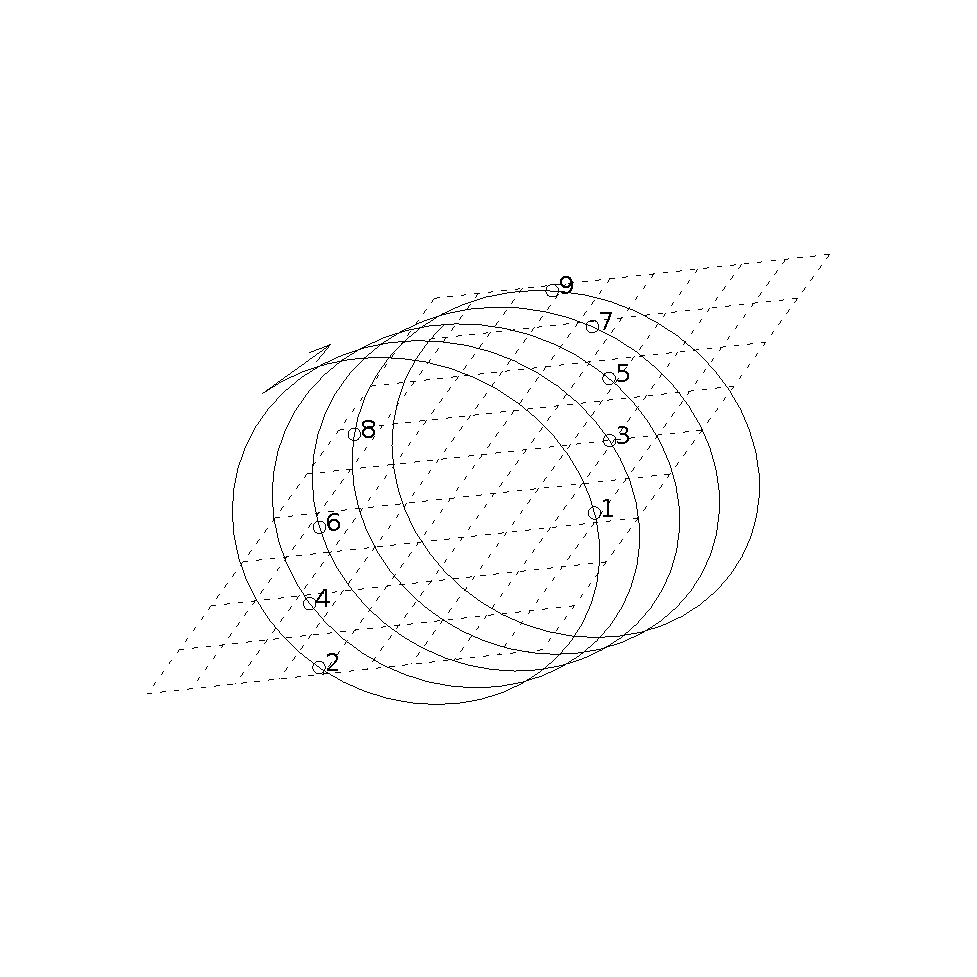
\includegraphics[trim={2.2cm 4cm 2cm 4cm},clip,width=.5,width=\textwidth]{images/arttrack/helix.eps}
         \caption{Винтовая линия, плоскость и точки пересечения в порядке
         заданном параметром $t$.}
         \label{fig:helixPlaneProblem}
     \end{subfigure}
     \hfill
     \begin{subfigure}[b]{0.6\textwidth}
         \centering
         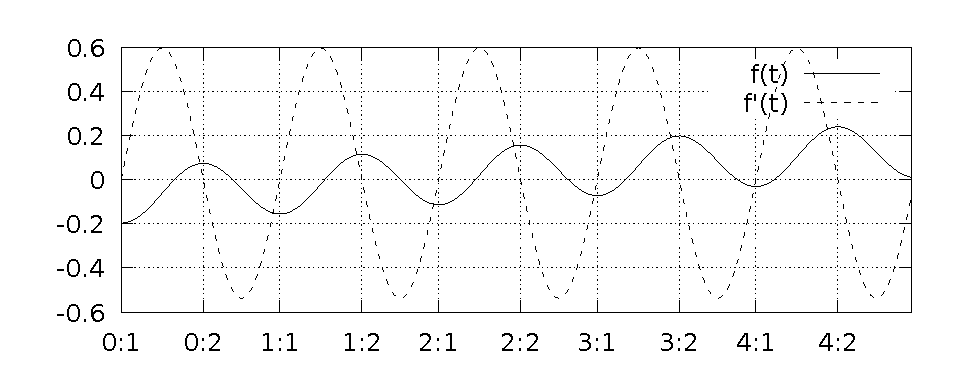
\includegraphics[width=\textwidth]{images/arttrack/helix-plane-func.eps}
         \caption{График функции проекции винтовой линии на нормаль плоскости.
         Отметки на горизонтальной оси соответствуют номеру периода и номеру
         экстремума в периоде.}
         \label{fig:hlxPlaneFuncAndDeriv}
     \end{subfigure}
        \caption{Изображение винтовой линии пересекающей плоскость и точек
            пересечения найденных при помощи численного метода в участках
            заданных \eqref{eq:helixPlaneExtrema}.}
        \label{fig:helixPlaneProblem}
\end{figure}

Для траектории заданной винтовой линией потребуется привлекать
численные методы, поскольку подстановка пропагатора \eqref{eq:helixMovement}
в уравнение плоскости приводит к трансцендентному уравнению с
произвольным числом корней
вида~$A \cdot \sin \theta + B \cdot \cos \theta + C \cdot \theta + D = 0$.
Участки монотонности этого трансцендентного уравнения заются двумя экстремумами
функции~\eqref{eq:helixMovement}:
\begin{equation}
    \theta_{1,2} = \pm \arcsin \frac{C}{\sqrt{A^2 + B^2}} - \arctan{\frac{B}{A}},
    \label{eq:helixPlaneExtrema}
\end{equation}
где $A = (\delta \vec{h} + \vec{t}_0) \cdot \vec{n}_p$,
$B = \alpha \vec{n}_p \cdot \vec{n}_0$, $C = \delta \vec{h} \cdot \vec{n}_p$.

Полностью, алгоритм отыскания пересечения винтовой линии
заданной~\eqref{eq:helixMovement} и плоскости выглядит следующим образом:
\begin{enumerate}
    \item Для заданного магнитного поля $\vec{B}$ импульса~$\vec{p}$ и
    заряда~$q$ частицы, отыскать экстремальные точки проекции касательного
    вектора на нормаль заданной плоскости~$\vec{n}_p$
    согласно~\eqref{eq:helixPlaneExtrema}, где $s > s_0$.
    \item Если корни \eqref{eq:helixPlaneExtrema} не определены (случай
    ориентации плоскости перпендикулярно полю), отыскание пересечения можно
    произвести численным методон последовательных приближений (напр. методом
    Ньютона), начиная с $s_0$.
    \item Подстановкой~\eqref{eq:helixPlaneExtrema} в~\eqref{eq:helixMovement}
    определить участки перемены знака и использовать в них численный метод
    отыскания нуля на отрезке (напр. дихотомий). При этом, если подстановка
    корней не приводит к уменьшению абсолютной величины среднего значения
    функции в течении двух последовательных периодов, считать, что пересечений
    с плоскостью нет (частица удаляется от плоскости).
\end{enumerate}
Реализация такого алгоритма должна предусматривать случай когда ось винтовой
линии
\begin{equation}
    \vec{l}(s) = \vec{r}_0 + \delta \vec{h} s + n_0 \alpha / K.
    \label{eq:helixAxis}
\end{equation}
параллельна плоскости --- то есть число корней~\eqref{eq:helixPlaneExtrema}
бесконечно.

Результат работы такого алгоритма представлен на рисунке~\ref{fig:helixPlaneProblem}.

\subsubsection{Определение локальных координат}

\begin{center}
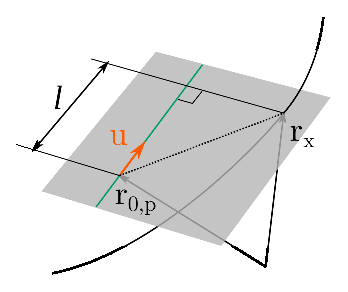
\includegraphics[width=.5\textwidth]{images/arttrack/arttrack-u-measurement.eps}
\end{center}

\subsubsection{Реализация}

\begin{figure}[ht]
    \centering
    \subfloat[Фронтальный вид]{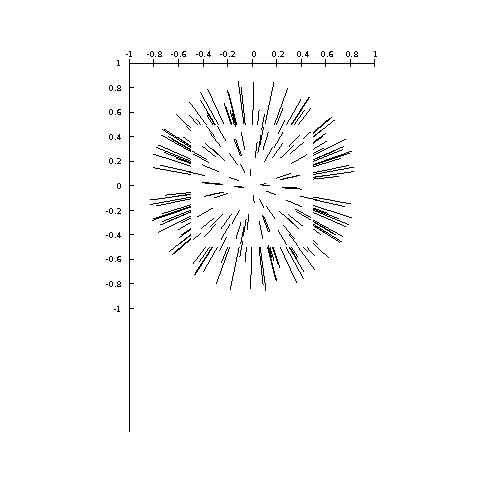
\includegraphics[trim={0 3cm 0 0},clip,width=.5\textwidth]{images/arttrack/box-in-sphere-ortho.eps}}
    % ^^^ trim={0 3cm 0 0},clip,
    \subfloat[Ортографическая проекция]{
\includegraphics[width=.33\textwidth]{images/arttrack/box-in-sphere.eps}}
    \caption{Визуализации различных тестов.}
    \label{fig:boxInSphere}
\end{figure}

